\documentclass[12pt]{book}
\usepackage[explicit]{titlesec}
\usepackage{lmodern}
\usepackage{lipsum}
\usepackage[a4paper,top=2.5cm,bottom=2cm,left=2cm,right=2cm]{geometry}
\usepackage[T1]{fontenc}
\usepackage[utf8]{inputenc}
\usepackage{graphicx}
\graphicspath{ {images/} }
\usepackage{lscape}
\usepackage[english,italian]{babel}
\usepackage{hyperref}
\setcounter{tocdepth}{2}\graphicspath{ {images/} }

\let\cleardoublepage\clearpage
\newlength\chapnumb
\titleformat{\chapter}[block]
{\normalfont\sffamily}{}{0pt}
{\parbox[b]{\chapnumb}{
   \fontsize{120}{110}\selectfont\thechapter}
  \parbox[b]{\dimexpr\textwidth-\chapnumb\relax}{
    \raggedleft
    \hfill{\LARGE#1}\\
    \rule{\dimexpr\textwidth-\chapnumb\relax}{0.4pt}}}
\titleformat{name=\chapter,numberless}[block]
{\normalfont\sffamily}{}{0pt}
{\parbox[b]{\chapnumb}{
   \mbox{}}
  \parbox[b]{\dimexpr\textwidth-\chapnumb\relax}{
    \raggedleft
    \hfill{\LARGE#1}\\
    \rule{\dimexpr\textwidth-\chapnumb\relax}{0.4pt}}}

\title{RASD Document (Requirements and Analysis Specification Document}
\author{Alessandro Negrini \and Andrea Gulino \and Paolo Guglielmino}
\date{October 2014}

\begin{document}
\selectlanguage{english}

\tableofcontents

\newpage
\vspace*{30cm}
\chapter{Introduction}
This document aims to provide a detailed analysis of the requirements and specifications related to the system we are going to develop. \\
Together with the Project Planning document, this will be the starting point of our work.\\
The Project Planning document allows us to better organize tasks in order to avoid loss of time and improve efficiency.\\
This document goes the same way, but doing it from a more technical perspective.\\
It is the first significant stage of the software lifecycle  (planning, development, design, testing, ... )\\ \medskip

The following is addressed to the team members and to every stakeholder involved in the project.\\
We will use it through all the development process in order to keep coherence with the specifications and satisfy all the requirements. Stakeholders, instead, will use it as a reference point to interpret our work.\\
Thus RASD is one of the most important gears of the entire engine and every defect of design could seriously affect the project success.\\ 
This is just the first version, changes and integrations could follow in the next deadlines.\\ \medskip

We start with a description of the problem in terms of the Jackson and Zave approach (The world and the Machine) and then we will go across the analysis of both functional and non-functional requirements.\\
We will make use of the usual UML formalisms, that include class diagrams, use cases, sequence diagrams and so on.\\
The final part will be devoted to the formalization and testing of our model made using Alloy.\\

\section{Description of the given problem}

The goal is to project and implement MeteoCal, a weather based online calendar.\\This software must help people to schedule their activities or events avoiding bad weather conditions if the activity is outdoor.\\There are two categories of users, those who are registered and those who are not. In order to use the functionalities provided by the software, the user must be registered.\\A non registered user can receive an invitation by a registered user, but in order to accept the invitation and take part to the event the user must register into the system.\\
Registered users can use the software to create, update and delete events (providing all the related information including where and when the events will take place, wether the event is indoor or outdoor,...).\\
The peculiarity of this application is that every event will be automatically enriched with weather forecast and the system will be able to notify the participants of the event in case of bad weather conditions, helping the users to find a proper solution. \\ \medskip

In addition, there are some other tasks that the system must accomplish: 
\begin{itemize}
	\item it has to provide a mechanism that allows people to make their own calendar public, so that it is visible to every other registered user. Users can decide whether to make public the entire calendar , or only the single event. In case of private event other users can only see that in those hours the user is busy.Otherwise if the events is public users also see events details. 
	\item a first way to propose a solution is the one in which the system, in case of bad weather, proposes to its creator three days before the closest sunny day when event can be organised. 
	\item the system must also provide a mail notification system (both for invitation and bad weather condition) 
	\item the system must provide a mechanism that allows users to export and import their calendar. 
	\item the system must avoid conflicts between events
	\item the system must periodically update weather conditions in order to keep track of weather changes and eventually notify users
\end{itemize}
\section{Definitions, acronyms, abbreviations}
Listed below are some definitions of those terms used inside the document that may cause ambiguity. \\ \medskip

\begin{tabular}{ |l|l| }
  \hline
  \hline
  \multicolumn{2}{|c|}{\large{\textbf{Dictionary}}} \\
  \hline
  \hline
  \textbf{Keyword} & \textbf{Definition} \\
  \hline
  Guest & It refers to the general guest of an event, both registered and\\& not registered\\
  World Phenomena & requirements engineering concerning with phenomena occurring \\&in the world.\\
  Machine Phenomena & requirements engineering concerning with phenomena occurring\\& in the machine.\\
  Shared Phenomena & phenomena that can be controlled by the world and observed by \\&the machine, or controlled by the machine and observed by the\\& world. \\
 Canceled Event & event that will not take place and is no more visible on the calendar \\
 Deleted Event & event deleted from system\\  
 Shared Event & event in which more than a user will take part \\
  \hline
  \hline
\end{tabular} \\ 
\vspace{0.5cm}

In addition we think that it can be useful to make having a glossary of abbreviations and acronyms:  \\ \medskip

\begin{tabular}{ |l|l| }
  \hline
  \hline
  \multicolumn{2}{|c|}{\large{\textbf{Glossary}}} \\
  \hline
  \hline
  \textbf{Acronym or Abbreviation} & \textbf{Definition} \\
  \hline
  \textbf{[WP]} & World Phenomena\\
  \textbf{[MP]} & Machine Phenomena\\
  \textbf{[SP]} & Shared Phenomena\\
  \textbf{[G]} & Goals\\
  \textbf{[A]} & Actors\\
  \textbf{[D]} & Domain Properties\\
  \textbf{[R]} & Requirements\\
  \textbf{[USC]} & USer Case\\
  \textbf{JEE} & Java Enterprise Edition\\
  \textbf{EJB} & Enteprise Java Beans\\
  \textbf{CSS} & Cascading Style Sheet\\
  \textbf{HTML} & HyperText Markup Language \\
  \textbf{JSP} & Java Server Pages\\
  \textbf{JSF} & Java Server Faces\\
  \textbf{DD} & Design Document\\
  \textbf{RASD} & Requirements Analysis and Specification Document\\
  \textbf{AJAX} & Asynchronous JavaScript And XML \\
  \textbf{HTTP} & HyperText Transfer Protocol \\
  \textbf{API} & Application Programming Interface \\
  \textbf{WAI} & Web Accessibility Initiative \\
  \textbf{W3C} & World Wide Web Consortium\\
  \hline
  \hline
\end{tabular} \\

\section{Overview}
What above was just a brief introduction to the project. In the following chapters things will be explained more deeply. 
However here we provide in advance a global view of document organisation : 
\begin{itemize}
	\item{\textbf{Chapter 2} \\ The second chapter starts giving a first idea of the proposed system, even if the detailed architecture will be shown in the Design Document. Then risks that can occur during the development are taken into account jointly with constraints. \\ Follows the identification of stakeholders and their relations with the system. \\ Another important part is represented by the Jackson and Zave approach, and problem is explored also under that perspective. \\ A fundamental part follows, one of the most important of all document and it is represented by preliminary considerations. \\
	The chapter ends with a collection of goals and domain properties, and thus the requirements derived from them.}
	\item{\textbf{Chapter 3}}\\ This section concerns with actors identifying, so that we point out everyone (or everything) who has to deal with system. In order to find actors, we ask ourselves which groups or user are supported by MeteoCal to perform their work. Eventually we show external hardware or software interact with the system. \\
	\item{\textbf{Chapter 4}}\\
	Non functional requirements specify criteria that can be used to judge the operation of a system, rather than specific behaviours. \\ We will define what our system is supposed to be ( not to do, covered by functional requirements). \\ 
	\item{\textbf{Chapter 5}}\\
	"Scenario is a narrative description of what people do and experience as they try to make use of computer system and applications"\footnote{M.Carrol, Scenario-Based Design, Wiley, 1995}.\\
	So in this part some significative informal descriptions of single system feature of the system used by a single actor are provided \\
	\item{\textbf{Chapter 6}}\\
	In this chapter we make use of UML diagrams in order to build system use cases and to express the flow of events. \\ Furthermore, a global static view of the system will be given using a Class Diagram. 
	\item{\textbf{Chapter 7 and 8}}\\
	Provide the alloy model contributed to the requirement analysis and analysis model. \\
	\item{\textbf{Chapter 9 and 10}}\\
	Used tools and references
\end{itemize}

\chapter{Overall Description}
Concerning the development of the front-end of this application we were allowed to choose between a java application and a web application.\\
We opted for the latter, convinced that this choice will bring benefits both to the development process and to user experience, especially considering the context of our application.\\ \medskip

	First of all, regarding the developing process, the application will have to interact with one or more external services through their APIs.\\ 
Most of modern APIs, such as Google APIs and forecast API we're going to use, are designed to easily fit the HTML5 paradigm. Moreover, JavaScript and its extensions (JQuery, AJAX) extremely simplify the integration with those services, reducing the code for an API request to just a bunch of lines.\\
Thus, the communication between the front-end and the back-end of our application will be connectionless, and the front-end will interact with the back-end in the same way it interacts with the other external services, that is through the use of an API.\\
Data exchange will be based on HTTP requests and XML data exchange; this will make the back-end completely independent from the front-end technology.\\ \medskip

	The second motivation regards the user experience. Users, should be able to use the application in any kind of situation, either when they are using their laptop/desktop computers but also, and probably mainly,  when they are outdoor using their personal tablets or smartphones.\\
Portability is nowadays one of keys to success for any kind of application. Even if java has been designed to be cross-platform, its portability is mainly limited to laptops and desktop computers. Web apps, instead, can be executed on any kind of device running a web browser. Moreover, they are always up-to-date and they behave almost the same way no matter the device, without being affected by system or software updates. Finally,  the large availability of open source templates and UI frameworks for web app development will allow us to build an awesome and scalable user interface, providing the best look and feel for any context of use.\\

\section{Risk Analysis}
During the problem analysis, we identified some risks that could compromise system development. 
First, requirements can be misunderstood and this could lead to errors or delays that could compromise the entire project . Therefore we have to be really careful to the requirements collection phase. \\ In addition, some stakeholders may not understand or feel confused reading them, thus a very important part is covered by formal modelling that allows readers to learn requirements in a better way, reducing ambiguities.
Another challenge consists on learning JEE jointly with the project development;  this could involve possible delays and additional efforts. \\
\section{Constraints}
Constraints to be satisfied can be divided in two categories: 
\begin{itemize}
	\item{\textbf{Software constraints: }system must be developed using JEE platform, and for business logic we are forced to use EJB. Other programming languages are not fixed in stone, but developing a web application means that we are implicitly asked to use languages such as HTML, CSS, Javascript, JSP, JSF, ... .\\ Users must have an up to date browser and an Internet connection. A more detailed description about software and hardware will be found further and in the next document, concerned with Design. }\\
	\item{\textbf{Time delivery constraints: } we are asked to meet some milestone and to deliver some documents for each of them : \\
	\begin{itemize}
    		\item 2 November 2014: Group registration and presentation\\
   		\item 16 November 2014: RASD Document ( we will attach also a not requested document, the Project Plan Document )\\
		\item 7 December 2014 : DD, that must contain a functional description of the system\\
		\item 25 January 2015 : Implementation following requirements and design specified in RASD. Source code and executable must be delivered, including installation document and user manual. In addition a detailed document where are indicated the number of hours spent by each group member \\
		\item 10 February 2015 : acceptance testing documentation realised on an other project developed by another group\\
		\item Date to be defined : final presentation, we can consider it like a deployment of the complete system 
  	\end{itemize}	 
	}
\end{itemize}

\section{Identifying stakeholders}
Our main stakeholder is the Professor, who wants to have a complete and working system that meets every specification provided with the problem.  
Her main goal is to check that we have understood the development process in all its parts and that we can carry out a project following each development phase taking care of milestones. \\
So we want to show that we can accomplish all these things, trying to provide a good quality documentation and of course a good quality software. \\
We will provide all base actions trying to extend the software with some extra functionality. \\ 
\vspace{0.2cm}

Another figure that can have a meaningful interest in the application is the end user. The user should be the most generic possible, so our software will be able to meet all kinds of usage. \\
Relating stakeholders to their interest into a table we can get the so call stakeholders matrix. Since we have just few stakeholders we get a non complete table. \\ 
\vspace{0.5cm}
\begin{center}
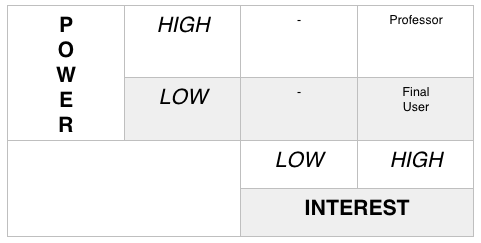
\includegraphics[scale=0.6]{matrix}\\
\end{center}
In order to satisfy the customer with a well developed application we pointed out three main aspects that we consider important: 

\begin{itemize}
	\item \textbf{Usability :} we want to put the user, rather than the system, in the centre of the process. Our system must be easy to use, but at the same time it must provide all functionalities. In order to reach this goal, our system will display its contents in a concise and clear way, building a simple and user friendly UI. \\ 
	\item \textbf{Nice User interface : } even if design isn't our main objective, we think that a good looking and endearing UI is essential to affect users.   \\
	\item \textbf{Stability : } system must be always available, and able to offer all its services. For example we should avoid possible system failures during registration process,  event creation and so on.\\
\end{itemize}

\section {The World and the Machine(Jackson and Zave)}
Up to now, we have presented the project from a general perspective, taking care of general aspects without using any formal model or language. \\ From now on, we start taking care of details, beginning with an high level abstraction: the World and the Machine model. \\ It was presented in 1995 by Jackson and Zave and it helps us to collect requirements, dividing them into three categories: World, Machine and Shared Phenomena. \\
We attached also an instance of the approach, even if this is not complete.\\ Its main goal is to show how these phenomena are related each others. \\

Just an instance of Jackson and Zave model\\
\begin{center}
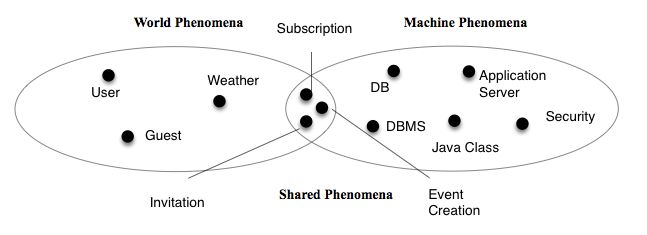
\includegraphics[scale=0.6]{JZ}
\end{center}

A more detailed list of phenomena

\begin{itemize}
	\item \textbf{World Phenomena} 
		\begin{enumerate}
			\item [WP1] : a general user decides to register into the system\\  
			\item [WP2] : weather changes \\
			\item [WP3] : a user decides to remove his account\\
			\item [WP4] : the event takes place \\
			\item [WP5] : a user decides to organise a new event \\
		\end{enumerate}
	\item \textbf{Machine Phenomena}
		\begin{enumerate}
			\item [MP1] : system deals with user registration\\  
			\item [MP2] : system stores user information in a secure DB\\
			\item [MP3] : system stores user events into a specific data structure \\
			\item [MP4] : system takes care of privacy policies  \\
			\item [MP5] : system finds a solution in case of bad weather for an outdoor event \\
			\item [MP6] : system provides a DBMS in order to manage DB\\
			\item [MP7] : every software that is part of the system (Application Server, ... ) \\
		\end{enumerate}
	\item \textbf{Shared Phenomena}
		\begin{enumerate}
			\item [SP1] : user fills in the registration form and signs up \\
			\item [SP2] : user creates a new event\\
			\item [SP3] : user invites some guest to one of his events\\
			\item [SP4] : guest receives an invitation\\
			\item [SP5] : guest decides to accept/decline invitation\\
			\item [SP6] : user removes his account from the system\\
			\item [SP7] : user sets event preferences \\
			\item [SP8] : user chooses a solution proposed by the system in case of bad weather\\
		\end{enumerate}
\end{itemize}

\section{Preliminary Considerations}

Before listing domain properties, since there are some points that are not so clear inside problem specifications, in this section we will make some assumption that will be respected during the overall project. In particular we assume that : 
\begin{itemize}
	\item An user can have \textbf{only one calendar}. This choice was driven by two reasons.\\ The first one is because we think that giving the user the opportunity to create more than one calendar does not make sense: a physical user can't be in two different place at the same time. \\The second is to simplify calendar management. In fact, if we suppose that a user can have more than one calendar (let us suppose 2, one for work and one for home), each time he adds an event the system should perform a double check: either verifying that there are no time conflicts within the same calendar, but also checking for time conflicts with events belonging to the other calendar.\\ 
	\item We assume that weather notifications are sent to the user only for outdoor events with an additional constraint. When users create an event, in addition to specifying wheter it is outdoor or not, they can set a notification trigger.\\ 
	The user receives notifications if and only if the event is outdoor and the expected weather is equal or worse than the weather specified setting the notification trigger.  \\ 
	The relation between API weather status and MeteoCal weather status id the following: \\
	- 0 : clear sky, few clouds = SUN\\
	- 1 : scattered clouds, broken clouds = CLOUDS\\
	- 2 : shower rain, rain = RAIN\\
	- 3 : thunderstorm = THUNDERSTORM \\
	- 4 : snow, mist = SNOW\\
	\item Non-registered users can be invited by registered users through their email address. In order to accept and use system functionalities they must register into the system with the same email address used for the invitation.  \\
	\item In order to develop a more complete and interactive software, we will allow guests to leave a comment to the event they have been invited to. \\
	\item Concerning with the way how the software will find the best solution in case of bad weather during an outdoor event, we have identified different policies to deal with this problem: \\ 
		        - starting from event creation moment, the system periodically updates the related weather information and whenever\\ a weather change is detected it notifies the user accoarding to what said before about the trigger; \\
			- three days before the event date, in case of bad weather, the system\\ notifies the user with a list of available time slots in which the weather is expected to be better.\\
			- in any case, the user can change the event time slot, cancel the event or simply ignore the notification.\\
	Visual representation of weather notifications : 
	\begin{center}
		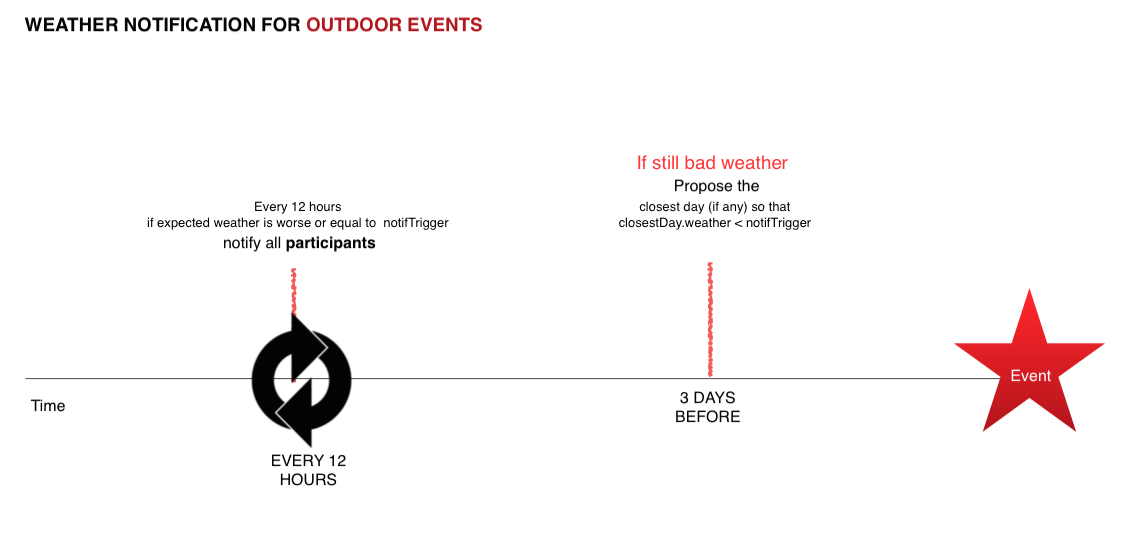
\includegraphics[width=16cm,height=8cm]{time}
	\end{center}
	
	\item We will introduce some social networking functions: users will be able to follow other users ( like in Twitter ), comment an event, view other users' profile and calendar (if public)
	\item The system will avoid time confilicts: not two events at the same time. \\ 
	\item Making calendar public, does not imply to have all events in it public.\\
	\item If event creator cancels a shared event all participants receive a notification followed by a note explaining the reason of cancellation \\
	\item If event creator changes date,time or place of an event, all participants receive a notification. \\ In this case all the users who had accepted the invitation are asked again to confirm their partecipation. \\
	\item Notifications are received only for outdoor events. \\
	\item All time references in DB are expressed as GMT+0. Time in user calendar is represented according to the user's default location. 
	\end{itemize} 
\vspace{5cm}
\newpage
\section{Goals}

The minimum set of features that the system should provide to its users is the following:\\ 

	\begin{tabular}{ |l|l| }
  		\hline
  		\hline
  		\multicolumn{2}{|c|}{\large{\textbf{Goals Table}}} \\
  		\hline
  		\hline
  		\textbf{Goal} & \textbf{Definition} \\
  		\hline
  			\textbf{[G1]} & Registration of a generic user\\
 		 	\textbf{[G2]} & User must be able to create a new calendar\\
			\textbf{[G3]} & User must be able to schedule its events inside his calendar\\ & avoiding bad weather conditions\\
			\textbf{[G4]} & CRUD operations on events must be supported\\
			\textbf{[G5]} & Users must be able to invite some guests to their events\\
			\textbf{[G6]} & Guests must be able to receive invitations by other users \\
			\textbf{[G7]} & The system must provide a mechanism in order to allow users to publish\\& their calendar\\
			\textbf{[G8]} & System must allow users to import and export their calendars\\
			\textbf{[G9]} & Users can either accept, decline or ignore an invitation \\
			\textbf{[G10]} & Users must be allowed to update and remove their accounts\\
			\textbf{[G11]} & System provides a solution in case of events problems \\&(bad weather conditions) \\
			\textbf{[G12]} & In order to manage events in a better way, system must update\\& weather condition periodically\\
			\textbf{[G13]} & Users must be allowed to view other users' public calendars \\ 
			\textbf{[G14]} & System must provide a way to specify weather preferences \\ 
			\textbf{[G15]} & For every modification to a shared events, all participants must\\& receive a notification\\
  		\hline 
  		\hline
	\end{tabular}  
\vspace{8cm}
\newpage

\section {Domain Properties}
The following is a list of domain conditions that should always be satisfied: \\

\begin{tabular}{ |l|l| }
  		\hline
  		\hline
  		\multicolumn{2}{|c|}{\large{\textbf{Domain Properties Table}}} \\
  		\hline
  		\hline
  		\textbf{Domain } & \textbf{Definition} \\ 
  		\hline
  			\textbf{[D1]} & A user can invite both registered and not registerd users\\
 		 	\textbf{[D2]} & A user doesn't have two overlapped events in the same hours. Even an overlap \\ & of a minute generates a conflict\\
			\textbf{[D3]} & A user doesn't invite the same guest at the same event more than once. \\
			\textbf{[D4]} & Weather forecasts provided by the open source weather data are correct \\
			\textbf{[D5]} & Users are uniquely identified by their email address \\
			\textbf{[D6]} & Users that attend an event have previously accepted an invitation to that event \\
			\textbf{[D7]} & Users that create an event or accept an invitation to a event participate to it \\
			\textbf{[D8]} & The system notifies participants to an event in case of bad weather at maximum\\ & one day before the event \\
			\textbf{[D9]} & The time slot in which a user decides to place his event is free and available \\
			\textbf{[D10]} & A user can't schedule an event for a past date/time\\
			\textbf{[D11]} & A user can't create events that end before they start, or events that last less \\ &than a minute. The same constraints must hold also when events are modified\\
			\textbf{[D12]} & A user can't invite himself\\
			\textbf{[D13]} & A user can invite both followed users and other users\\
			\textbf{[D14]} & A user can't follow himself \\
			\textbf{[D15]} & A public calendar doesn't imply that events inside it are public as well \\
			\textbf{[D16]} & In order to make an event public, the calendar in which it is placed must\\&be public\\
			\textbf{[D17]} & Only the user who created the event can update, cancel or delete it\\
  		\hline 
  		\hline
	\end{tabular} \\ 

\section{Functional Requirements}

Starting from domain properties, written in the previous section (section 2.7), supposing that they hold and taking in consideration goals ( section 2.6 ), we can derive the following requirements. \\

The table in the next page is designed so that for each goal (assumed that domain properties hold) we derive the most important requirements that the system must meet.  \\

\begin{tabular}{ |l|l| }
  		\hline
  		\hline
  		\multicolumn{2}{|c|}{\large{\textbf{Requirements Table}}} \\
  		\hline
  		\hline
  		\textbf{ } & \textbf{Derived requirements } \\ 
  		\hline
  			\textbf{[G1]} & 
					-\textbf{[R1]} The system has to provide a sign up functionality  \\&
					-\textbf{[R2]} The system updates the DB with correct data \\
			\textbf{[G2]}  & 
					-\textbf{[R3]} The system creates, for each registered user, one associated calendar \\&
					-\textbf{[R4]} The system can allow user to delete and recreate a new calendar from 						scratch\\	
			\textbf{[G3]} & 
					-\textbf{[R5]} The system provides an interface in order to allow user scheduling their					events\\&
					-\textbf{[R6]} The system provides a mechanism that is able to avoid events during bad\\& weather conditions\\&
					-\textbf{[R7]} The system updates weather forecasts periodically\\&
					-\textbf{[R8]} The system provides weather information during the event creation process \\
			\textbf{[G4]} & 
					-\textbf{[R9]} The system provides CRUD operations for events\\
			\textbf{[G5]} & 
					-\textbf{[R10]} The system allows users to find other user's profiles\\&
					-\textbf{[R11]} The system offers the possibility to invite guests to events\\&  
					-\textbf{[R12]} The system proposes a list of followed users when a user \\ &wants to make invitations\\
			\textbf{[G6]} & 
					-\textbf{[R13]} The system collaborates with a SMTP server in order to send\\& email notifications\\&
					-\textbf{[R14]} The system offers an ad hoc internal mechanism to notify users in addition\\& to email \\  
			\textbf{[G7]} & 
					-\textbf{[R15]} During event creation, the system provides an interface that allows\\& users to choose whether the calendar/event is public/private\\
			\textbf{[G8]} &
					-\textbf{[R16]} During events creation system must check that the new event doesn't\\& overlap with another\\
			\textbf{[G9]} &
					-\textbf{[R17]} The system must be able to upload and import external calendars\\& 
					-\textbf{[R18]} The system must be able to export the user calendar in different formats\\ 			\textbf{[G10]} &
					-\textbf{[R19]} The system provides a way to accept or decline invitation\\
			\textbf{[G10]} &
					-\textbf{[R20]} The system has a module that manages user settings and allows users\\& to remove or update their account.   \\
			\textbf{[G11]} &
					-\textbf{[R21]} The system provides different policies to find a solution in case of bad\\& weather conditions for outdoor events. As explained in section 2.5,\\& system allows user to change date ( so the system looks for the closest \\& good weather day presenting to the user the possible choices ), or to change place.  \\ &As for changing place, the user can choose a new place manually, \\ & or can rely on a system tool that suggests him the most suitable place . \\
			\textbf{[G12]} &
					-\textbf{[R22]} The system allows all the partecipants to an event to leave a comment\\& on that event\\
			\textbf{[G14]} &
					-\textbf{[R24]} During event creation, the system lets the user to choose a custom \\& notification trigger \\
			\textbf{[G15]} &
					-\textbf{[R25]} The system includes a mail notification mechanism\\&
					-\textbf{[R26]} The system also allows users to display notifications within the application UI\\
  		\hline 
  		\hline
	\end{tabular} \\

\chapter{Actors Indentifying}

The actors of the system represent all those entities that interact in an active way with the system. We found three different kind of actors that interact with the system: 
\begin{itemize}
	\item \textbf{ A1] NOT REGISTERED USER } : not yet registered user. 
		\begin{itemize}
			\item He can register into the system, so he becomes a registered user\\
			\item He can receive invitation from other registered user\\
		\end{itemize}
	\item \textbf{ A2] USER } : registered user   
		\begin{itemize}
			\item He can schedule his calendar\\
			\item He can create/update/cancel/delete his events\\
			\item He can browse other user public calendars \\
			\item He can follow other users \\
			\item He can accept or decline invitations \\
			\item He can comment events he is invited to \\
			\item He can update or delete his profile \\
			\item He can log into the system\\
			\item He can logout \\
		\end{itemize}
	\item \textbf{ A3] SYSTEM ADMINISTRATOR } : the system manager. 
		\begin{itemize}
			\item He can have a complete access to the system\\
			\item He can manage user profiles \\
			\item He can manage the overall system \\
			\item He can manage preferences regarding weather forecasts update routines \\
		\end{itemize}
\end{itemize}

If we agreed with the Use Case formalism that considers as an actor any external hardware or software interacting with the system, we should have considered as an actor also the external service that provides weather forecasts to the MeteoCal. \\
Anyway, we opted not to consider this system as an actor because, at this level of abstraction, we think that we can consider it as a part of our system, and not as an external component.   

\chapter{System Quality}
\section{Non functional Requirements}

Non functional requirements refer to "what the system shall be". They describe the interaction between the system and its environment independently from implementation.\\
We have pointed out some non functional requirements that system must meet, and also some qualities that our development will guarantee.\\ We already mentioned some of them in section 2.3, here we provide a complete detailed list.
	\subsection{Usability and Portability}
		 As already told our system will provide an easy to use graphic interface. Moreover, we want that our software can be used on the largest possible number of devices. Thus, our platform must be well designed both for desktop and smartphones. Thus, the front-end must be developed in a way that allows to fit all screen sizes. \\ 
		In addition, we expect to provide a mobile implementation of this application. This extra project is carried on within another university course : Design and Implementation on Mobile Application.  \\ It won't be a web app application, but an application developed using ad hoc mobile programming language in order to improve and offer some functionalities that a simple web app wouldn't be able to offer.\\
	\subsection{Accessibility}
		Accessibility is the degree to which our application is available to as many people as possible. We can consider it as the 'ability to access'. \\ Often, this concept focuses on people with disabilities or special needs (blind people, ... ) . \\
		A member of our group last year, within a international context (Athens programme), attended a course of "Accessible Web Design" and he will put in action all the things he learned. \\
		Overall we will try to meet the rules imposed by WAI and W3C standards \\ 
	\subsection{Efficiency}
		Within software development framework, efficiency means to use as less resources as possible. \\ Thus, system will provide data structures and algorithms aimed to maximize efficiency. \\ 
		We will also try to use well known patterns reusing as many pieces of code as possible, taking care of avoiding any anti-pattern. \\ 
	\subsection{Extensibility}
		Our system must provide a design where the implementation takes future growth into account. It will be developed in a way such that the addition of new functionalities won't require strong changes to the internal structure and data flow. \\
	\subsection{Maintainability}
		As in the section above, when a developer will have to fix something inside the code, the implementation will try to make the maintenance operation easy to accomplish.\\
	\subsection{Availability and Stability}
		Our system must be able to offer its services whenever the user asks for them. It must be available 24/7.\\
		In case of malfunctioning, administrator will provide maintenance in order not to affect service availability\\
	\subsection{Security/Privacy}
		Without any doubt it is one of the most important requirements. \\ Every online service that deals with personal data should ensure this property. Supposed that data is permanent on the disk, system must concern with privacy of data. In order to meet this requirement, it will provide an authorization system that filters only registered users. \\
		Users' Passwords are collected in a secure and encrypted way on a database. In this way the user will be the only person knowing his passwords. \\ 
		Not only the database must be secure, but also every transaction between front-end and back-end should rely on secure protocols ( Actually, since building a secure protocol costs money, we suppose that classical protocols will ensure security). 
	\subsection{Reliability}
		Since data are exchanged among users, data reliability is essential. Users can base their actions on other users' data. Moreover, we suppose that the memory where database is stored is stable. 
\section{User Interfaces}
The interface of our application is though to be used via internet, in order to reach the most part of the users in every way. \\
As yold before, MeteoCal will provide a simple and complete graphic structure that makes it easy to find main functionalities by users. \\
What follows are some page layouts according to which our UI will be designed.\\
Our platform contains two main environments, one is about user profile management, and the other one is about event management within which the user can have a look to his calendar and perform actions like adding new event, delete, update, and so on. \\

\subsection{Login interface}
\begin{center}
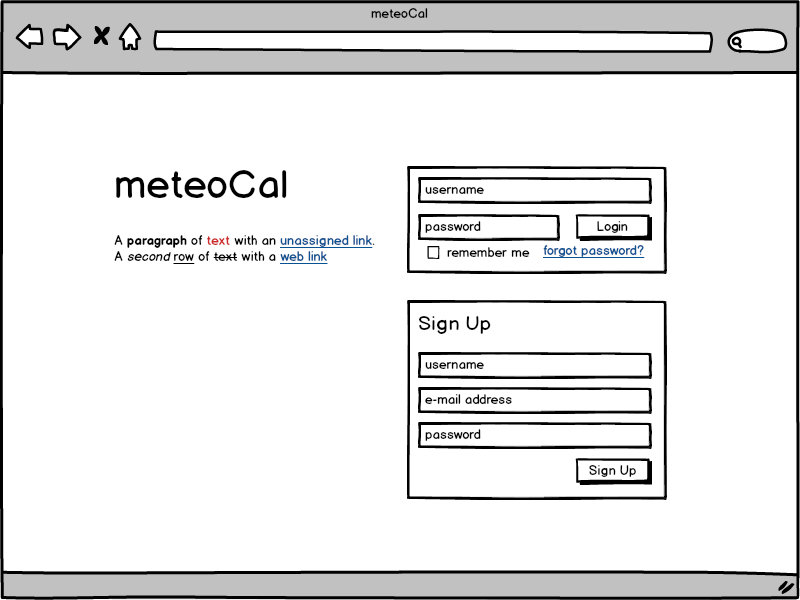
\includegraphics[scale=0.4]{mockup_home}
\end{center}
\subsection{User Profile interface}
\begin{center}
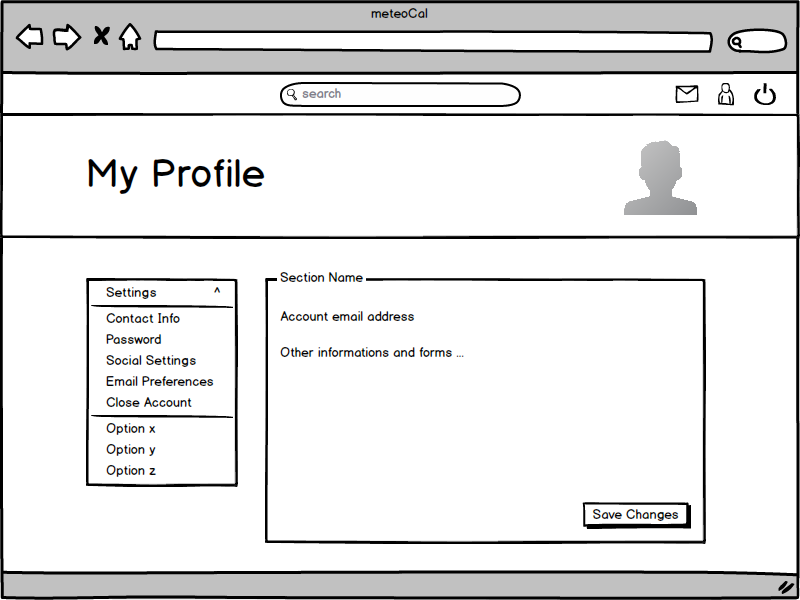
\includegraphics[scale=0.4]{mockup_profilesettingpage}
\end{center}
\subsection{Calendar interface}
\begin{center}
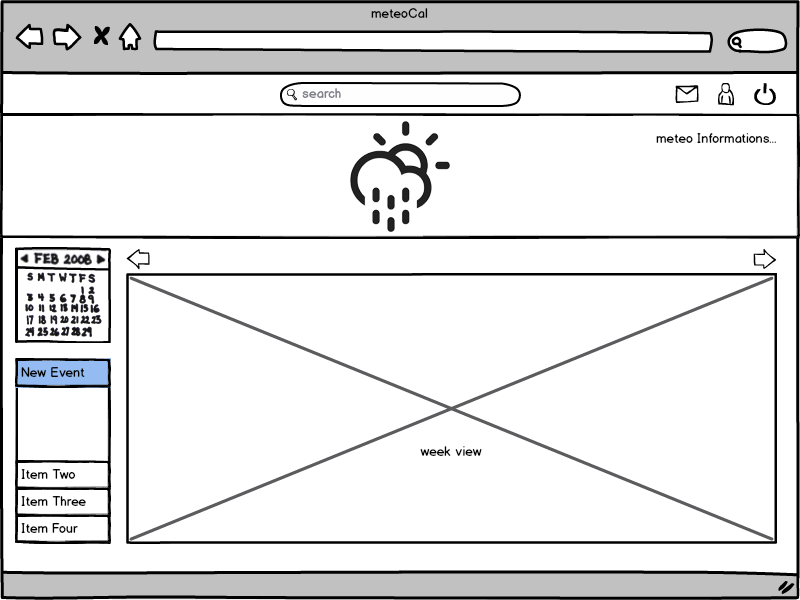
\includegraphics[scale=0.4]{mockup_calendarpage}
\end{center}
\subsection{Create Event interface}
\begin{center}
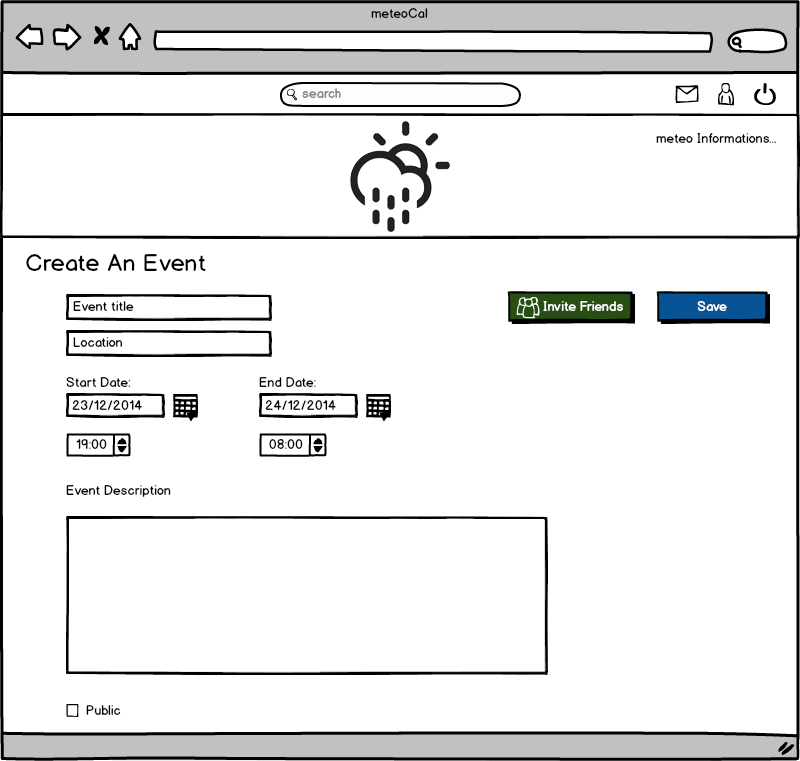
\includegraphics[scale=0.4]{mockup_createEvent}
\end{center}

\section{Documentation}
In order to show project development and also to offer a documentation to the final user, we will write the following documents: 
\begin{itemize}
	\item \textbf{Project Plan} : defines team members and team organization. A brief time estimation will be done.
	\item \textbf{RASD} : addressed to final users, clients, analysts and developers. Its objective is to understand the given problem defining its goals, requirements and specification
	\item \textbf{DD} : addressed to developers and analysts. It aims to define real structure of our web application and its tiers. 
	\item \textbf{JavaDoc comments in the source code}: addressed to other developers in order to understand and maintein the code. 
	\item \textbf{Installation Manual }
	\item \textbf{User Manual} 
	\item \textbf{Testing Document}: report of a project developed by another group
\end{itemize}

\section{System Architecture}
We have already given a quite detailed explanation of our system . Here we point out the main components used.\\ 
From the server side point of view, since our platform is developed over a JEE platform, JSP and Servlets are fundamentals.
As for the client side, the final user only needs to have a browser.\\

\chapter{Scenarios Identification}

In this part of the document we will provide, starting from requirements specified in an a natural language, partially detailed in previous chapters, a brief description of the system using some scenarios. Afterwards, we will come up with a higher level description through use cases, using also a semi-formal notation: UML diagrams.\\ \medskip

Known the size of our project, we could list hundreds of scenarios. The list below states just some of them.

\section{Alice decides to register to the system}
Alice's life is very busy and she looks for a system that allows her to schedule her activities. Moreover, she wants the system to provide a mechanism of notifications that is able to keep her up to date on event changes. \\
So she googles for "Agenda" and she gets a wide list of results. Scrolling down she finds the result  "MeteoCal" and she wonders why that agenda has that name. She decides to click on it and the home page, containing a brief description of the app functionalities,  appears. She reads the description and she gets captured by the fact that the application joins the agenda with weather forecasts. She thinks that in that way whenever she wants to do something outside she can rely on it. Thus, she decides to register to the system, she fills-in and submits the registation form with her personal information, including also a default location, and confirms her email address by clicking a link eclosed in the received email that finally redirects her to the app login page. \\ 

\section{Alice starts scheduling an event with her children to the sea}
After loggind-in, Alice starts scheduling her activities trying to create a new event for the next Sunday afternoon. So she presses "New event" and an empty form is shown.\\
She has to provide the name of the event, when it starts and it ends, a brief description, and choose between the "outdoor" and "indoor" options. Her event is an outdoor one, and when she sets the "outdoor" option, she notes with pleasure that, differently from other agenda software that she previously tried, she can also add her weather preferences. \\Since she expects to go to the seaside with her children, she specifies that she wants to be notified only in case of rainy weather. In case of clouds, she will go to sea anyway.\\
Finally she presses the "Add" button and the event is correctly added to her calendar.\\

\section{Bob plans a shared event with three friends}
Bob is a man who has already discovered MeteoCal before Alice did. He uses it very often and today he wants to plan Saturday night outside with other three friends. He decides to create an event with guests on MeteoCal. So he creates an event and he specifies all event information and weather preferences. Before pressing the "Add" button, in order to confirm event, he invites his friends, so he types two of his friends' names  and he adds the suggested users to the event, and adds the email of a friend who is not registered to MeteoCal. Finally, he presses the "Add" button and the event is correctly added to his calendar. \\

\section{Alessandro, a registered user, receives the invitation from Bob and accepts}
Alessandro, the first of the three persons that Bob invited to his event, is scheduling a picknic with his family for next Friday afternoon.\\ He is logged into the system and at a certain point he ears the MeteoCal notification sound, it is Bob's invitation. \\
He opens the notification and gets redirected to the invitation. After looking at the event details he clicks on the 'Acceot' button and the event is finally added to his calendar. 

\section{Andrea unfortunately can' t attend the event}
Andrea, the last of the three persons that Bob invited to his event, is working hard on his PhD thesis of Philosophy and he considers ephimeral going outside with other friends. While he is writing his thesis on his 'brand new' Windows 98, he receives an invitation email by MeteoCal. \\
Opening the link enclosed in the email and logging in into the system, he reads about Bob's event invitation but, for the reasons explained above, he is is forced to decline the invitation. When he declines the invitation, he has also the opportunity to explain the reason why he has declined it, and he writes a brief note apologizing with Bob, Alessandro and Paolo. 

\section{Paolo, a non registered user, receives the invitation from Bob and accepts}
Paolo, the third of the three persons that Bob invited to his event, is surfing on internet when he receives an email from MeteoCal. He isn't registered to the application. \\ He is interested to Bob invitation and he wants to accept after checking the event date and time. He pressed the "Accept " button on the received mail, and the MeteoCal registration page appears.\\ Paolo fill in the form with his information, and finally he can accept and confirm his participation to the event. At the end his calendar has a scheduled event for the saturday night.\\ 

\section{Bob, the event creator, two days before the event, finds out a problem}
Two days before attending the event with his friends, Bob finds out that on Saturday night he isn't free and he must attend an appointment that he can't miss. \\
So he decides to postpone the event to the next week, using updating options provided by the system. \\
The System will notify his friends (the invited ones), including Andrea, the one that refused, because in this new date he could be available, sending them a notification .\\ The event is moved from the original Saturday, to the next one. \\

\section {Andrea gets available for the new date}
Andrea receives the notification that the date of the event has changed. \\
On that date he will have already discussed his thesis, and so he will be willing to attend the meeting with Bob, Alessandro and Paolo. After logging-in and accepting the invitation he is finally added to the invitation partecipants and a new event appears on its calendar. \\

\section{Paolo confirms the changes }
Also Paolo confirms changes and the event is rescheduled for the new date .

\section{Alessandro can't attend the modified event} 
On the contrary, Alessandro, who works in the city hospital, has to watch over his patients on that specific date time and so he is forced to decline the invitation. \\ He writes a note explaining the reason why he can't be present. 

\section{Alice updates her profile}
Alice suddenly remembers that her profile can be enriched with some more information, and she also wants to 
upload a profile photo. So she logs into the system and accessing to personal information manager section, she has the possibility to change all her data. 

\section{Alice receives bad weather notification and reschedules he revent}
Two days before the event, Alice receives a bad weather notification from MeteoCal. MeteoCal provides her a list of possible time slots for which she can reschedule the event. The first solution proposed is for the following Tuesday, but she can't do that because she is at work. Another proposed time slot is for the following Saturday. She's free and she chooses this option. \\
Her calendar is updated. 

\section{Marco receives bad weather notification and he ignores}
Marco is a user that has planned an outdoor event for Monday morning. The day before, he receives a bad weather notification, and as usual MeteoCal provides him some solutions. \\
Marco decides to keep his event anyway, so he ignores the notification. \\ The calendar remains unchanged.

\chapter{UML Models}
\section{Use Case Diagram}
Starting from scenarios collected in the previous section and the general analysis done at the beginning of this document, we could derive many use cases. However, we will do a detailed description, not for every possible use case, as done for scenarios, but only for the most significative ones . \\

Use cases are flows of events initiated by an actor. \\

First, we design a \textbf{Use Case Model}, that is the set of all use cases specifying the complete functionality of the system .\\ 

Then, each single use case is handled on its own. For each use case, information like use case name, participating actors, exceptions, flow of events and thus sequence diagram associated are provided. We describe in a detailed way the main use cases.\\ Some use cases that extend other use cases are omitted because they are really similar to others. \\ 

The use cases we are going to present are the following: 
\begin{itemize}
	\item{Sign up}
	\item{Log in}
	\item{Creation of new event}
	\item{Receive event request}
	\item{Make public calendar}
	\item{Updating event information}
	\item{Deletion event}
	\item{Updating personal profile}
	\item{Follow another user}
	\item{Event invitation}
	\item{Search a registered user and see his public events/calendar}
	\item{Account remove}
	\item{Calendar export}
	\item{Calendar import}
	\item{Provide a feedback to an event}
	\item{Add a new system functionality}	
 \end{itemize}

\subsection{Use Case Model}
Below the general use case is depicted, in it we include our main actors. 
It offers just a very high level vision of the system. 
\begin{center}
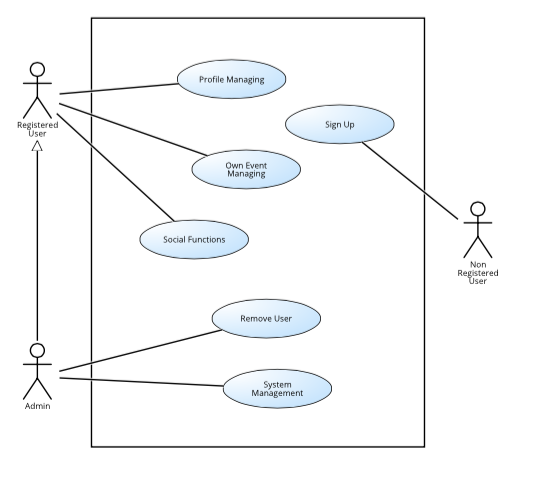
\includegraphics[scale=0.8]{generalUC}
\end{center}

We pointed out three main categories of use cases. We call them : 
\begin{itemize}
	\item Event Management : it collects functionalities like creation of a new event, event deletion, update event details, export calendar and import calendar
	\item Profile Management : it collects functionalities like login, registration, updating personal info, and account deletion
	\item Social : it collects functionalities like following new user, searching for user, viewing user's profile and calendars, rate and comment, receive event invitation. 
\end{itemize}

\subsection{Event Management Use Case}
\begin{center}
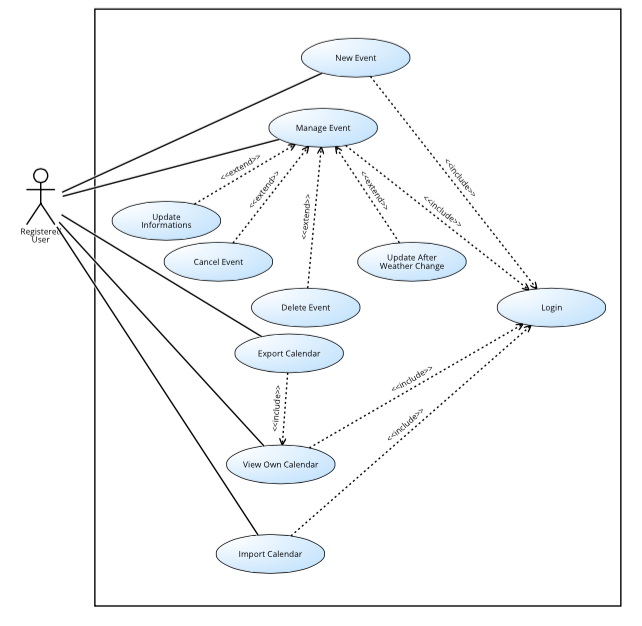
\includegraphics[scale=0.8]{eventManagementUC}
\end{center}
\subsection{Social Use Case}
\begin{center}
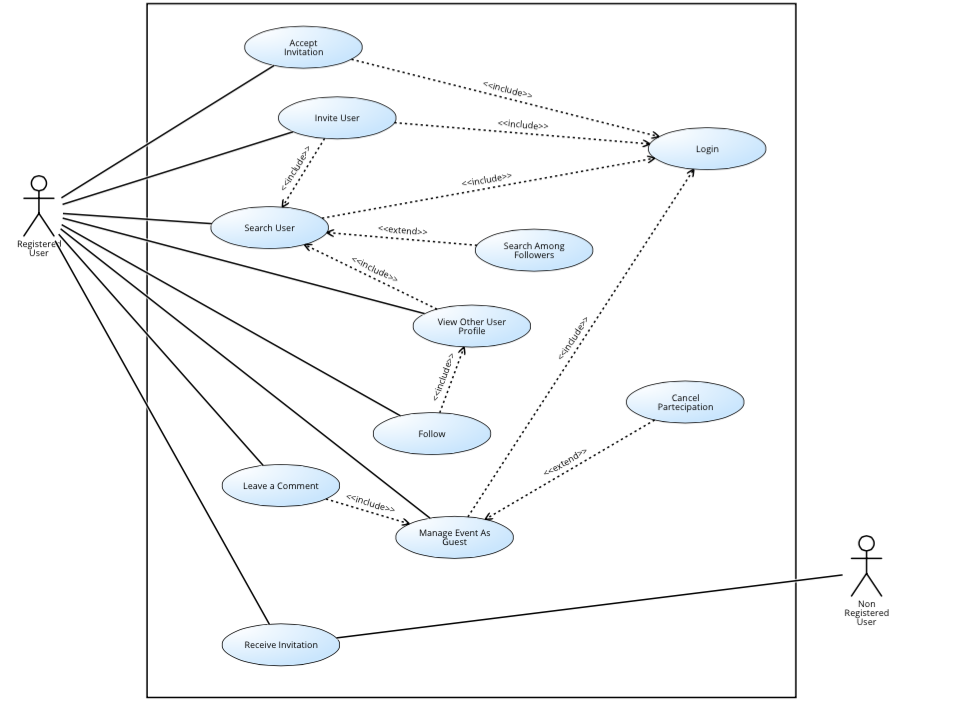
\includegraphics[width=20cm,height=13cm]{socialUC}
\end{center}
\subsection{Profile Management Use Case}
\begin{center}
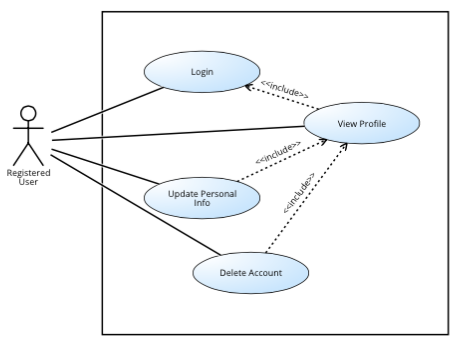
\includegraphics[scale=0.6]{profileManagementUC}
\end{center}

\section{Sequence Diagram}
\subsection{Sign up}
\begin{center}
\vspace*{\fill}
\begin{tabular}{ |l|l| }
  		\hline
  		\hline
  		\multicolumn{2}{|c|}{\large{\textbf{Sign up}}} \\
  		\hline
  		\hline
  		Code  & USC01\\ 
		\hline
		Description & The unregistered user registers in the system\\
		\hline
		Assumptions & The user is not registered yet\\
		\hline
		Actors & Non-registered user\\
		\hline
		Entry conditions & The user navigates to the homepage of MeteoCal\\
		\hline
		Exit conditions & Profile information and data are successfully saved. User is registered\\
		\hline
		Exceptions & User types something wrong, or misses to fill something. Email \\& address can be not unique. Users doesn't click on email\\& confirm\\
		\hline
		Flow of events & 
			1. The User opens the home page of MeteoCal \\&
			2. The System shows him the form to be filled in \\&
			3. The User clicks on register button\\&
			4. The System shows him the form to be filled in\\&
			5. The user inputs his personal information and click on confirm\\& button\\&
			6. The System checks data validity and uniqueness of the email address. \\&
			7. The System sends the confirmation email\\&
			8. The User clicks on confirm\\&
			9. The System creates profile and opens the log in page \\& Also a user calendar \\
  		\hline 
		Sequence Diagram &  \includegraphics[scale=0.5]{SignUpSD}\\
		\hline
  		\hline
\end{tabular} \\
\vspace*{\fill}
\end{center}
\subsection{Log in }
\begin{center}
\vspace*{\fill}
\begin{tabular}{ |l|l| }
  		\hline
  		\hline
  		\multicolumn{2}{|c|}{\large{\textbf{Log in}}} \\
  		\hline
  		\hline
  		Code  & USC02\\ 
		\hline
		Description & The registered user logs into the system\\
		\hline
		Assumptions & The user is registered to the system\\
		\hline
		Actors & Registered user or Administrator\\
		\hline
		Entry conditions & The user has successfully signed up to the system\\
		\hline
		Exit conditions & None \\
		\hline
		Exceptions & Username or password are wrong\\
		\hline
		Flow of events & 
			1. The User or administrator opens the home page of MeteoCal\\&
			2. The system shows him the page \\&
			3. The User or administrator inputs his username and password and  \\& clicks on log in button \\&
			4. The System checks data correctness\\&
			5. The System shows the profile or administrator page\\
  		\hline 
		Sequence Diagram &  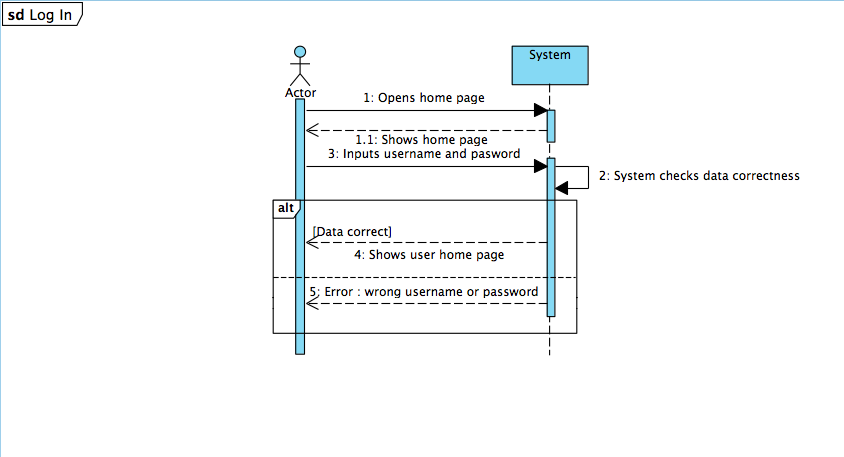
\includegraphics[scale=0.45]{LogInSD} \\
		\hline
  		\hline
\end{tabular} \\
\vspace*{\fill}
\end{center}

\subsection{Creation new event }
\begin{center}
\vspace*{\fill}
\begin{tabular}{ |l|l| }
  		\hline
  		\hline
  		\multicolumn{2}{|c|}{\large{\textbf{Creation new event}}} \\
  		\hline
  		\hline
  		Code  & USC03\\ 
		\hline
		Description & User creates an event\\
		\hline
		Assumptions & The user must be logged in, and he wants to create a new event that\\& doesn't already exist\\
		\hline
		Actors & Registered user\\
		\hline
		Entry conditions & The user has successfully signed up to the system\\
		\hline
		Exit conditions & The event is correctly created and scheduled on the calendar \\
		\hline
		Exceptions & New event generates a conflict with another event. \\
		\hline
		Flow of events & 
			1. The User clicks on event create button\\&
			2. The system shows him the section in which user fill in event\\& information \\&
			3. The User inserts starting and ending time and date, the name of the \\ & event, a note \\&
			4. The User confirms clicking on confirm button\\&
			5. The system checks for conflicts\\&
			6. The System schedule in the correct way the event on user's \\&calendar\\&
			7. The Systems redirects user to invite user page\\&
			8. The User selects user to invite\\&
			9. The System adds them to events and send a notification\\& [see receive event request]\\
  		\hline
		&\\
		Sequence Diagram &  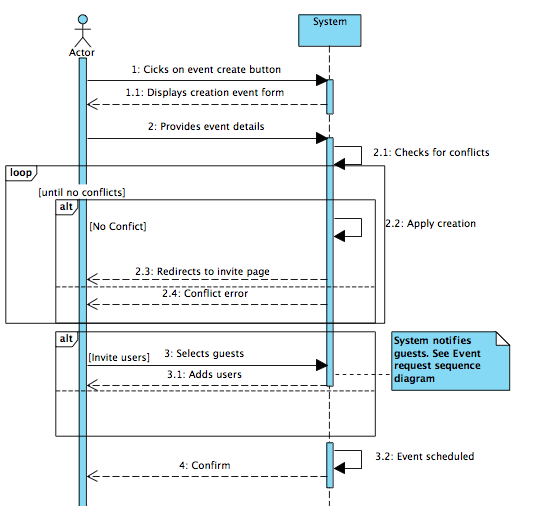
\includegraphics[width=12cm, height=10cm]{newEventSD}\\
		\hline 
  		\hline
\end{tabular} \\
\vspace*{\fill}

\end{center}

\subsection{Make Public Calendar}
\vspace*{\fill}
\begin{center}
\begin{tabular}{ |l|l| }
  		\hline
  		\hline
  		\multicolumn{2}{|c|}{\large{\textbf{Make Public Calendar}}} \\
  		\hline
  		\hline
  		Code  & USC04\\ 
		\hline
		Description & A user wants to make public his own calendar\\
		\hline
		Assumptions & The user must be logged in, and he wants to make his calendar public\\&
		Making calendar public, does not imply to have all events inside it\\ & public as well. \\
		\hline
		Actors & Registered user\\
		\hline
		Entry conditions & The user has successfully signed up to the system\\
		\hline
		Exit conditions & The calendar is visible to everyone\\
		\hline
		Exceptions & None \\
		\hline
		Flow of events & 
			1. The User clicks on his profile\\&
			2. The System displays his information\\&
			3. The Users switches the visibility settings of his calendar\\&
			4. The System performs the action and allows everyone to view it\\ &
			5. The System redirects user to home page \\
			
  		\hline 
		 &\\
		Sequence Diagram &  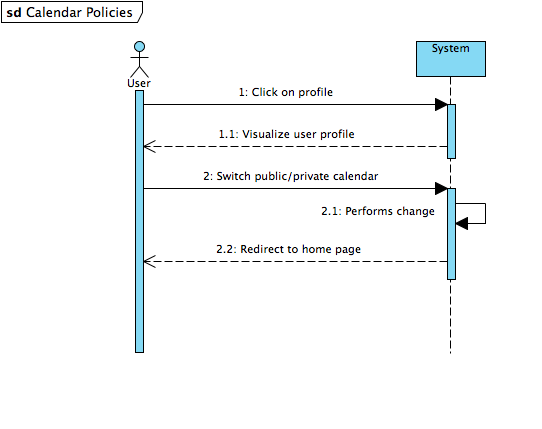
\includegraphics[width=12cm, height=12cm]{CalendarPoliciesSD}\\
		\hline
  		\hline
\end{tabular} \\
\end{center}
\vspace*{\fill}
\subsection{Receive event request}
\vspace*{\fill}
\begin{center}
\begin{tabular}{ |l|l| }
  		\hline
  		\hline
  		\multicolumn{2}{|c|}{\large{\textbf{Receive event request}}} \\
  		\hline
  		\hline
  		Code  & USC05\\ 
		\hline
		Description & User receives a invitation by an other user. This use case\\& describes only the relation between system and the invited user, when \\ & he receives an invitation. \\
		\hline
		Assumptions & User has a mail address\\
		\hline
		Actors & Registered or non-registered User\\
		\hline
		Entry conditions & An user has invited a user to attend his event\\
		\hline
		Exit conditions & User decides whether accept or decline the invitation\\ 
		\hline
		Exceptions & User ignores email invitation \\
		\hline
		Flow of events & 
			1. The System sends an email that invite the user to attend a particular event\\&
			2. The User decides whether accept/decline\\&
			3. The User logs into the system if he is already registered\\&
			[User signs up if he is not yet registered (see sign up use case \\&and sequence diagram)]\\&
			4. The System provides him an interface that allow user to choose whether \\ & accept/decline\\&
			5. The User clicks on accept/decline button\\&
			6. The System informs event creator user whether he accepted or not\\ 
  		\hline 
		&\\
		Sequence Diagram &  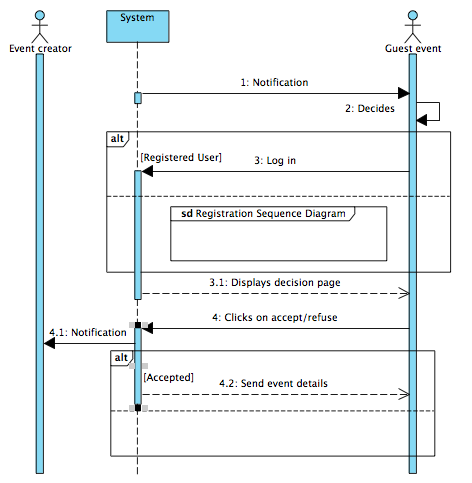
\includegraphics[width=11cm, height=10cm]{newEventRequestSD}\\
		\hline
  		\hline
\end{tabular} \\
\end{center}
\vspace*{\fill}
\subsection{Make event public}
\vspace*{\fill}
\begin{center}
\begin{tabular}{ |l|l| }
  		\hline
  		\hline
  		\multicolumn{2}{|c|}{\large{\textbf{Make event public}}} \\
  		\hline
  		\hline
  		Code  & USC06\\ 
		\hline
		Description &  A user wants to make public his own event\\
		\hline
		Assumptions & User has at least an event scheduled in calendar\\
		\hline
		Actors & Registered User\\
		\hline
		Entry conditions & User is logged into the system  \\
		\hline
		Exit conditions & The event details is visible to everyone \\
		\hline
		Exceptions & None \\
		\hline
		Flow of events &  
			1. The User clicks on one of his events\\&			
			2. The System shows events detail \\&
			3. The User switches event visibility setting \\&
			4. The System performs changes\\
  		\hline 
		&\\
		Sequence Diagram & 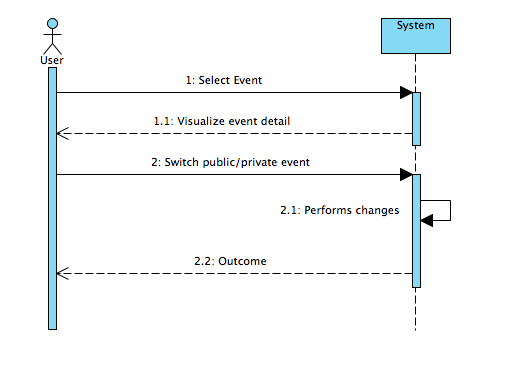
\includegraphics[width=12cm, height=10cm]{eventPoliciesSD}\\
		\hline
  		\hline
\end{tabular} \\
\end{center}
\vspace*{\fill}
\subsection{Update User profile}
\vspace*{\fill}
\begin{center}
\begin{tabular}{ |l|l| }
  		\hline
  		\hline
  		\multicolumn{2}{|c|}{\large{\textbf{Update User profile}}} \\
  		\hline
  		\hline
  		Code  & USC07\\ 
		\hline
		Description &  The user wants to update his profile ( photo, add tel.number, ...)\\
		\hline
		Assumptions & User is registered\\
		\hline
		Actors & Registered User\\
		\hline
		Entry conditions & User is registered and he is logged into the system\\
		\hline
		Exit conditions & User profile is updated \\
		\hline
		Exceptions & None  \\
		\hline
		Flow of events &  
			1. The User clicks on update profile button\\&	
			2. The System retrieves profile info\\&
			3. The System shows him the update form\\&
			4. The User changes or add some fields \\&
			5. The System updates the new profile \\ &
			6. The System sends notification to the User\\
  		\hline 
		Sequence Diagram & \includegraphics[width=13cm,height=9cm]{UpdateProfileSD}  \\
		\hline
  		\hline
\end{tabular} \\
\vspace*{\fill}
\end{center}

\subsection{User starts following an other user's profile}
\begin{center}
\vspace*{\fill}
\begin{tabular}{ |l|l| }
  		\hline
  		\hline
  		\multicolumn{2}{|c|}{\large{\textbf{User starts following an other user's profile}}} \\
  		\hline
  		\hline
  		Code  & USC08\\ 
		\hline
		Description &  User wants to add to his MeteoCal friends another registered user\\
		\hline
		Assumptions & User is registered\\
		\hline
		Actors & Registered User\\
		\hline
		Entry conditions & User is registered and he is logged into the system\\
		\hline
		Exit conditions & Users now is following that profile  \\
		\hline
		Exceptions & None  \\
		\hline
		Flow of events &  
			1. The Users search for a particular user searching him on search bar\\&			
			2. The System shows him his profile\\&
			3. The User clicks on follow button\\&
			4. The System adds a new profile to the ones that user already follows  \\
  		\hline 
		&\\
		Sequence Diagram &  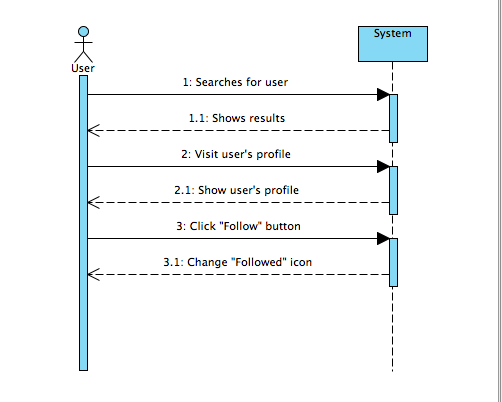
\includegraphics[width=13cm,height=9cm]{followSD}  \\
		\hline
  		\hline
\end{tabular} \\
\end{center}
\vspace*{\fill}

\subsection{User views another user's public calendar}
\vspace*{\fill}
\begin{center}
\begin{tabular}{ |l|l| }
  		\hline
  		\hline
  		\multicolumn{2}{|c|}{\large{\textbf{User views another user's public calendar}}} \\
  		\hline
  		\hline
  		Code  & USC09\\ 
		\hline
		Description & User wants another registered user's calendar\\
		\hline
		Assumptions & User is registered and the other has a public calendar\\
		\hline
		Actors & Registered User\\
		\hline
		Entry conditions & User is registered and he is logged into the system\\
		\hline
		Exit conditions & User has a view on public calendar \\
		\hline
		Exceptions & None  \\
		\hline
		Flow of events &  
			1. The Users search for a particular user searching him on search bar\\&			
			2. The System shows him his profile\\&
			3. The User clicks on button that allows him to view his calendar \\&
			4. The System shows him the complete calendar with eventually also \\ & public events\\
  		\hline 
		&\\
		Sequence Diagram & 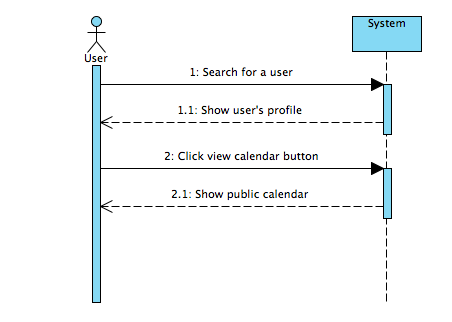
\includegraphics[scale=0.6]{viewUserSD}\\
		\hline
  		\hline
\end{tabular} \\
\end{center}
\vspace*{\fill}
\subsection{Bad Weather Notification}
\vspace*{\fill}
\begin{center}
\begin{tabular}{ |l|l| }
  		\hline
  		\hline
  		\multicolumn{2}{|c|}{\large{\textbf{Bar Weather Notification}}} \\
  		\hline
  		\hline
  		Code  & USC10\\ 
		\hline
		Description & System updates weather condition, and notifies user in case of bad weather\\
		\hline
		Assumptions & System receives weather updates\\
		\hline
		Actors & Registered and Non Registered User\\
		\hline
		Entry conditions & None \\
		\hline
		Flow of events &  
			1. The System updates weather conditions\\&	
			2. The System checks if there are outdoor events scheduled in bad\\& conditions\\&
			3. The System sends email notification to event creator and any invited \\& users
			4. The User takes a decision\\&
			5. The System reschedules the event with new details, if changed \\ &
			6. The System sends confirmation to any user\\
  		\hline 
		&\\
		Sequence Diagram & 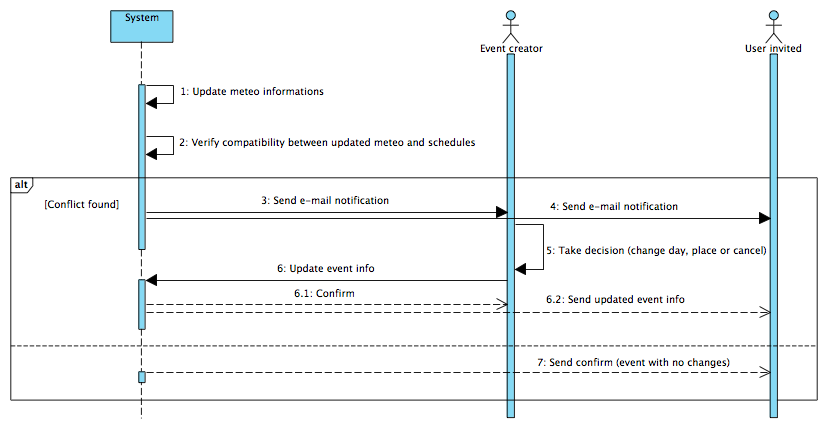
\includegraphics[width=13cm,height=11cm]{badWeatherSD}  \\
		\hline
  		\hline
\end{tabular} \\
\end{center}
\vspace*{\fill}

\section{Class Diagram}

Now it's time to derive, starting from requirements detailed in the previous chapter and flow of events, our project class diagram. It presents project specification under a static point of view of main entity involved in, and their relationship. \\
The following diagram introduces the conceptual classes that we have decided to include in the software product. 

\begin{landscape}
\begin{center}
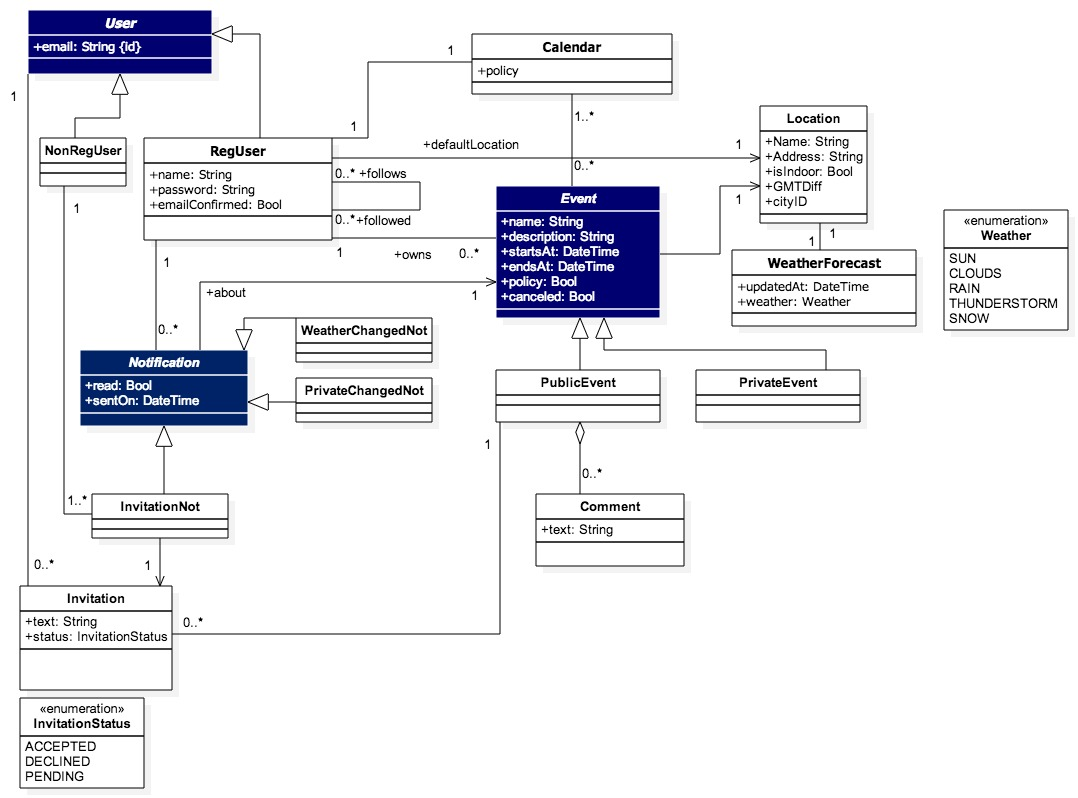
\includegraphics[width=25cm, height=16.5cm]{UML}\\
\end{center}
\end{landscape}

\section{State Charts Diagram}
\subsection{Lifecycle of an event}
At the beginning, when a user creates an event, the event is in "To be performed" state. Then if he doesn't cancel it, when the current time corresponds to the event starting time the events starts and so it goes into "On going state", until it ends and goes into "Passed" state.\\ Eventually, before the event starts, the user can cancel the event, and event goes into "Cancelled" state. \\
\begin{center}
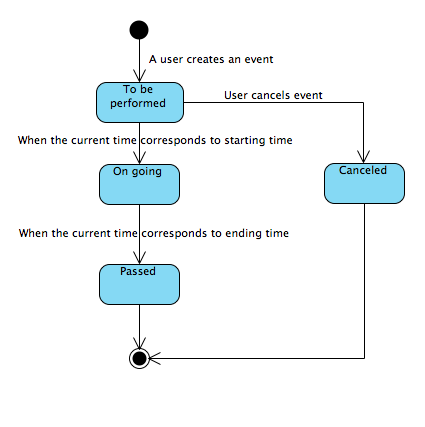
\includegraphics[scale=0.8]{eventSCD}\\
\end{center}

\subsection{Lifecycle of an invitation}
At the beginning, when a user creates a shared event, system sends a notification to a given user. The first state is the "Pending" one, that means that the invitation hasn't received an answer yet by invited user. \\
If invite is accepted/declined it goes into "Accepted"/"Declined" state.\\  
\begin{center}
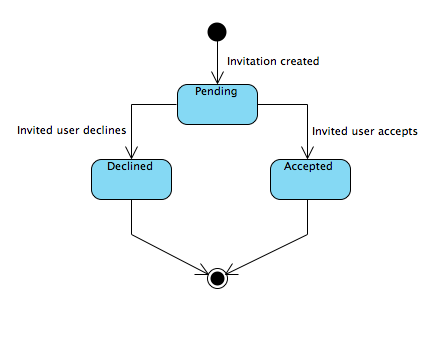
\includegraphics[scale=0.8]{invitationSCD}\\
\end{center}

\chapter{Alloy Modelling}
Our main goal is not be inconsistent, and now, using this tool we try to understand if our Class Diagram is well designed using Alloy Analyzer. \\
The following Alloy code models a system abstract representation. \\
\newpage
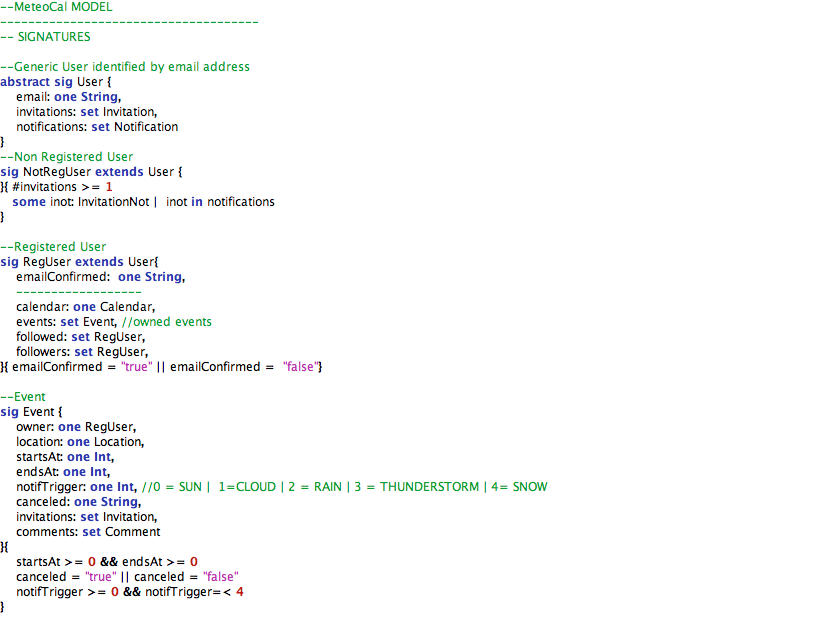
\includegraphics[width=19cm,height=21cm]{Alloy1}\\
\newpage
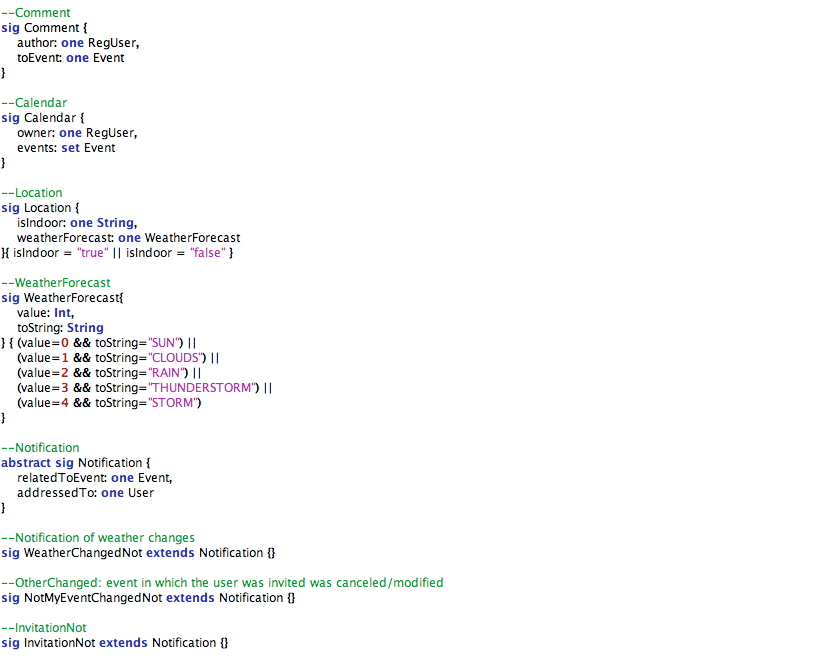
\includegraphics[width=19cm,height=21cm]{Alloy2}\\
\newpage
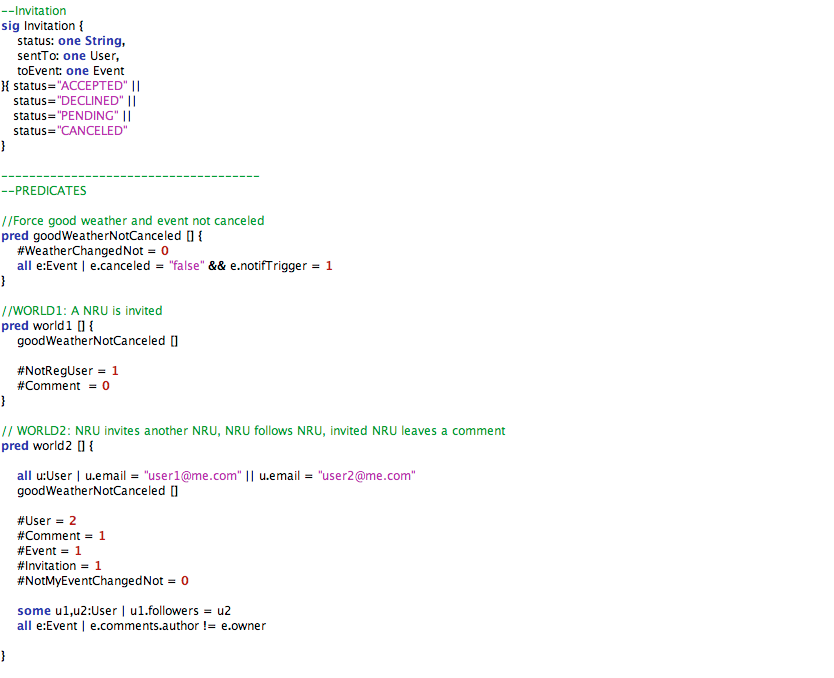
\includegraphics[width=19cm,height=21cm]{Alloy3}\\
\newpage
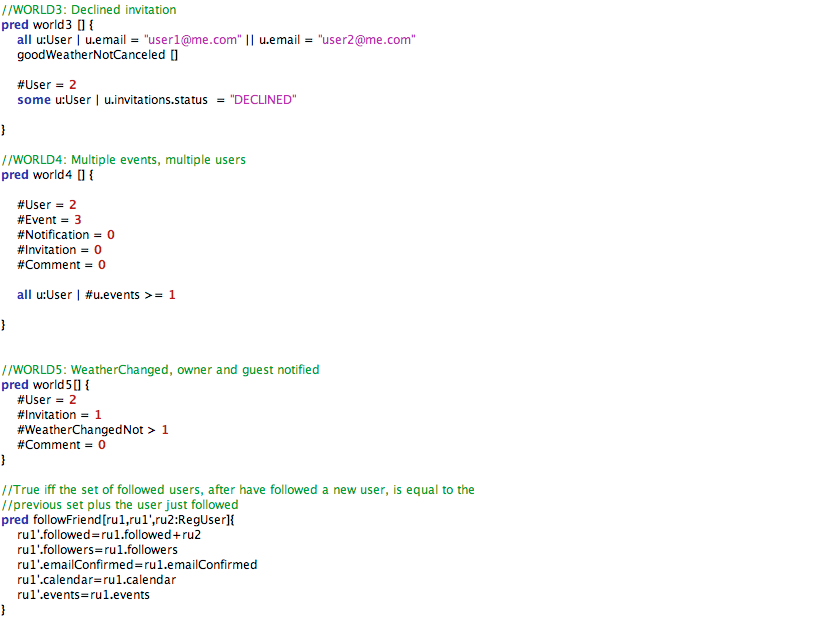
\includegraphics[width=19cm,height=21cm]{Alloy4}\\
\newpage
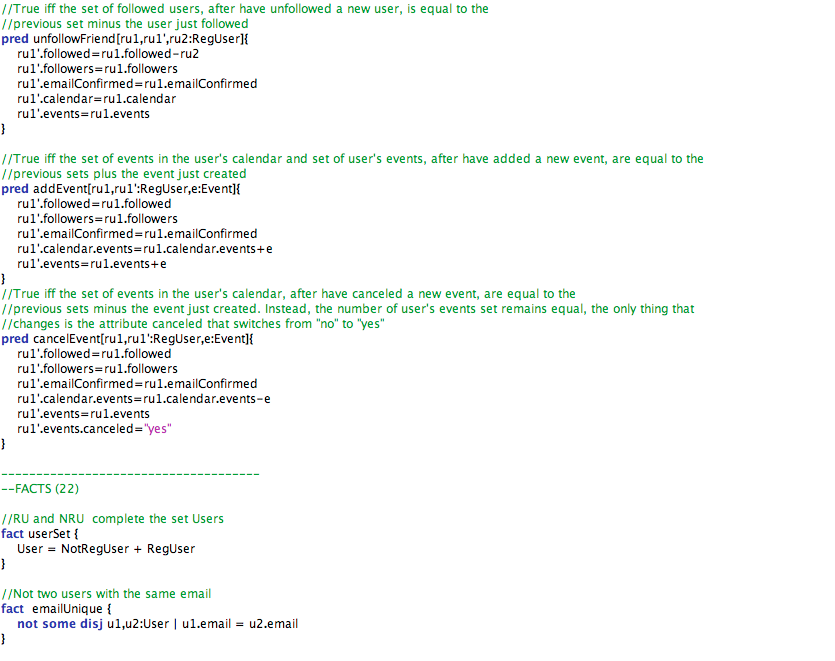
\includegraphics[width=19cm,height=21cm]{Alloy5}\\
\newpage
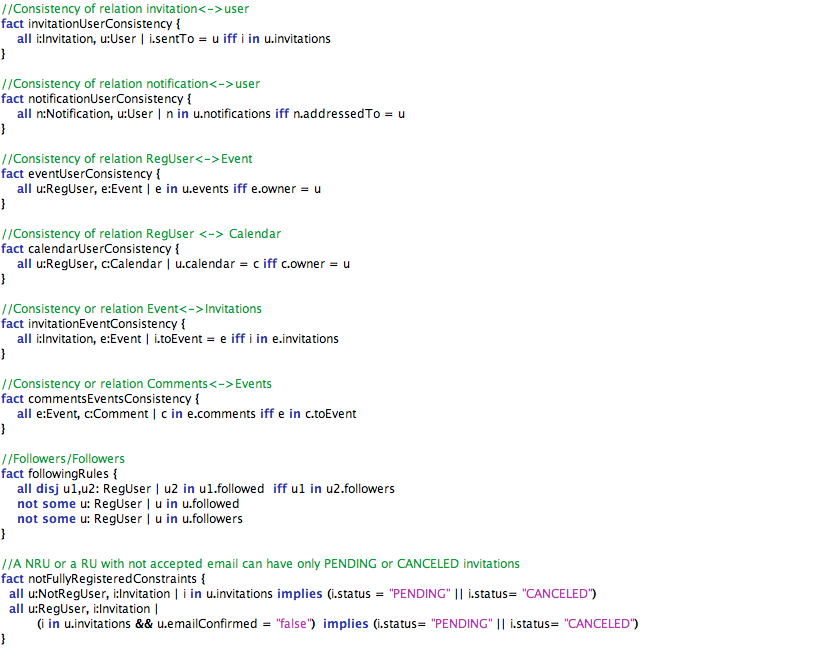
\includegraphics[width=19cm,height=21cm]{Alloy6}\\
\newpage
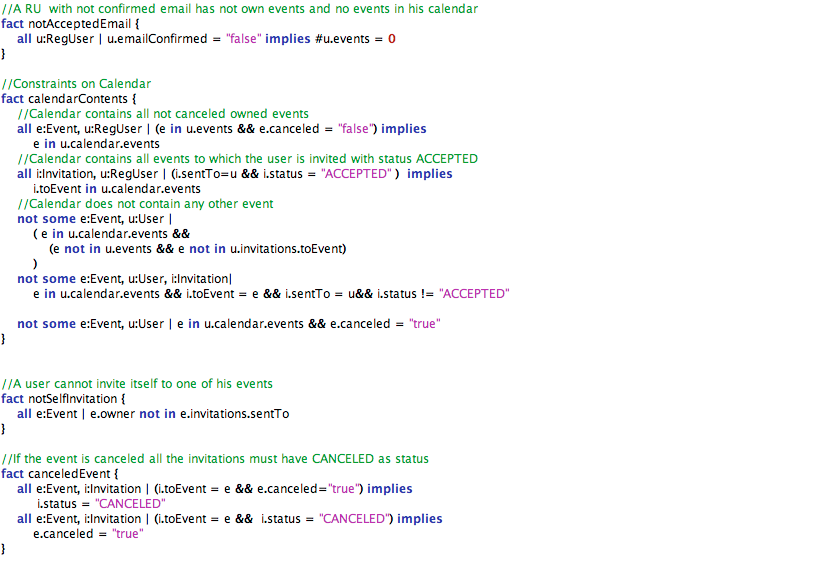
\includegraphics[width=19cm,height=21cm]{Alloy7}\\
\newpage
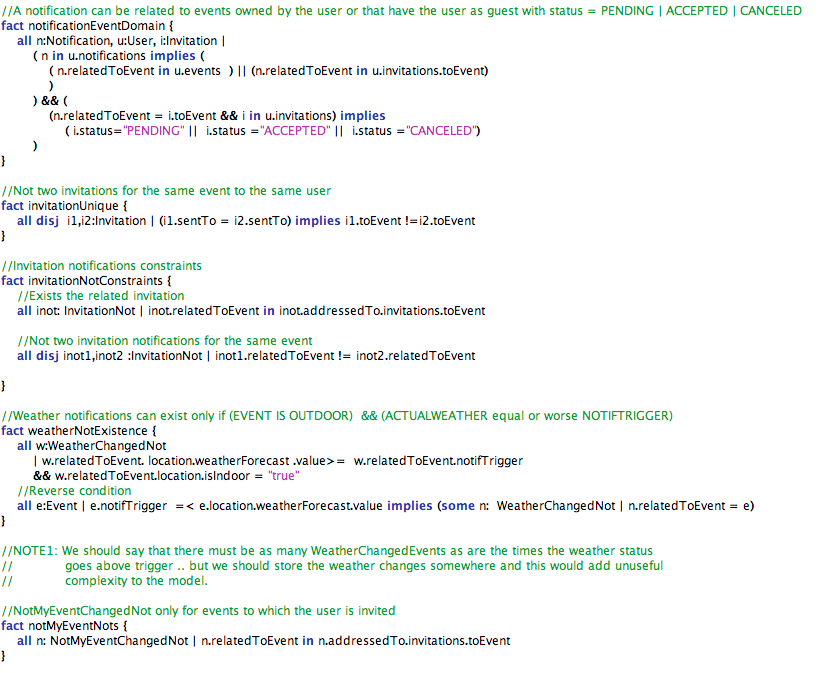
\includegraphics[width=19cm,height=21cm]{Alloy8}\\
\newpage
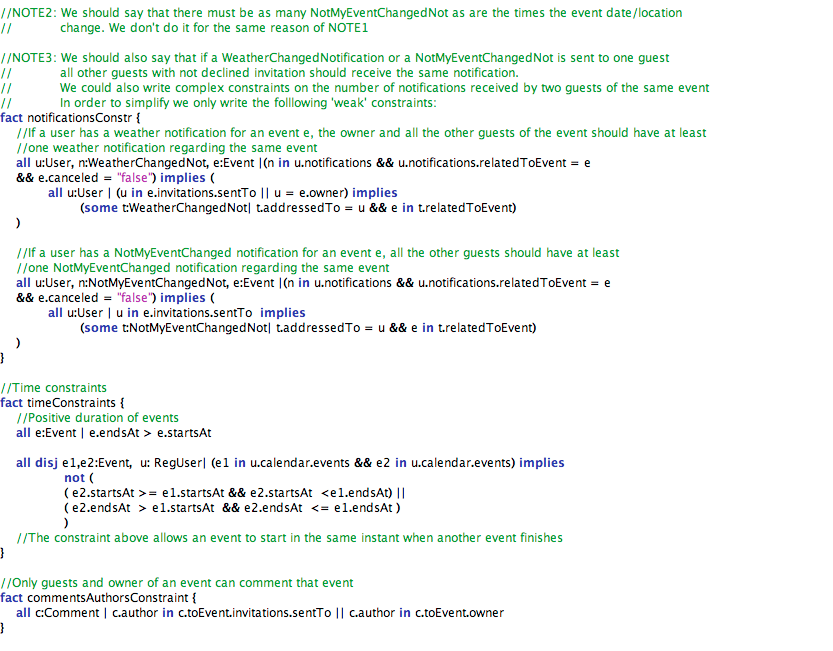
\includegraphics[width=19cm,height=21cm]{Alloy9}\\
\newpage
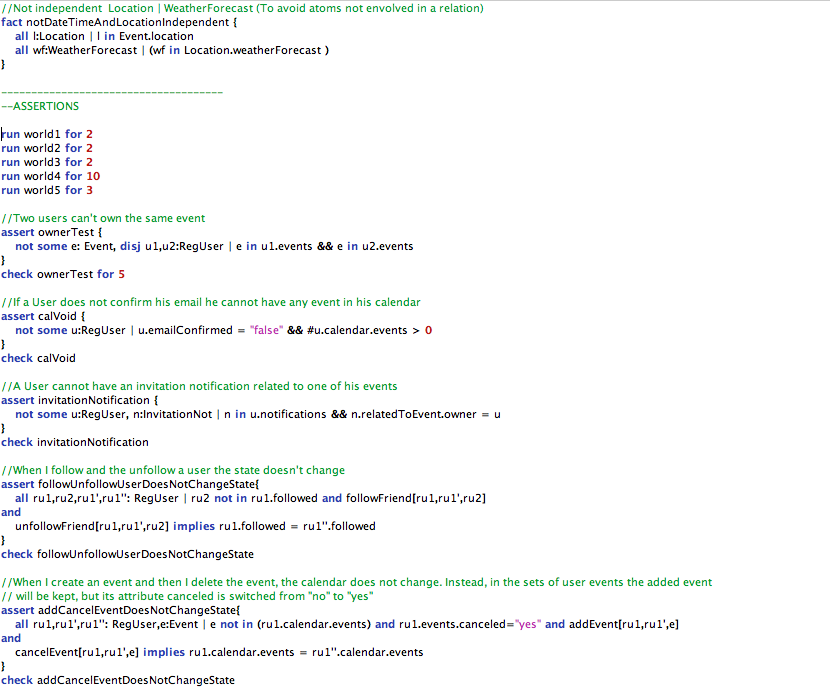
\includegraphics[width=19cm,height=21cm]{Alloy10}\\
\newpage
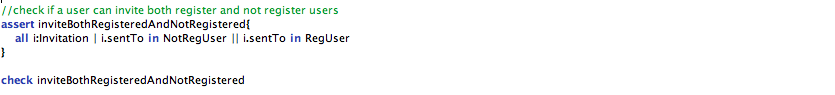
\includegraphics[scale=0.8]{Alloy11}\\

And here the report of the Alloy Analyzer : \\

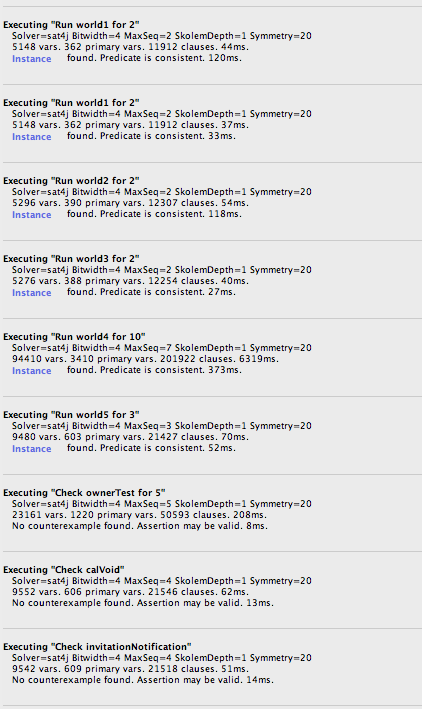
\includegraphics[scale=0.8]{result1}\\
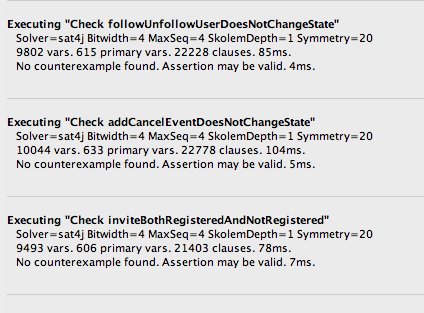
\includegraphics[scale=0.8]{result2}\\

\chapter{Worlds Generated}
\section{Not registered User World}
In this world, NotRegUser, who is not registered, is invited to an Event  created by RegUser, who is registered.\\
NotRegUser has an invitation to that event with status 'PENDING' and a Invitation notification related to the same event.\\
Some main constraints are satisfied:\\
- Not two users with the same email\\
- A NotRegUser can only have 'PENDING' or 'CANCELED' invitations\\
- A NotRegUser has no calendars / own events\\
- When there?s an Invitation there must be an associated InvitationNotification\\
- A not-canceled event appears in its owner's calendar\\
- If the event is not canceled there's no invitation to that event with status 'CANCELED'\\


\section{Invitation World}
In this world, RegUser1 follows RegUser0.\\
RegUser1 has created an Event and has invited RegUser0 to it.\\
Therefore RegUser0  receives an InvitationNotification and decides to ACCEPT the invitation.\\
Now the event appears on its Calendar1.\\
Eventually, RegUser0 leaves a Comment to the event.
Some important constraints are satisfied:\\
- If RegUser1 follows RegUser0, RegUser0 must be in RegUser1's followers\\
- Only users invited to an event can leave a comment to that event\\
- If an invitation is ACCEPTED, the related event must appear in the guest's calendar\\
- Not two invitations for the same event addressed to the same user\\

\section{Decline Invitation World}
In this world, RegUser0 invites RegUser1 to one of his events.\\
RegUser1 decides to DECLINE the invitation. Thus, the event won't appear in RegUser1's Calendar.
Remarkable constraints:\\
- If an invitation is DECLINED, the related event must not added to the invited user's calendar

\section{Events World}
In this world RegUser0 has created two events:\\
- Event1 starts at 5 and ends at 6\\
- Event2 starts at 6 and ends at 7\\
Both events are in RegUser0's calendar.\\
Another user, RegUser1 had an event Event0 starting at 0 and ending at 3, but he decided to cancel it.
Satisfied constraints:\\
- An event can be owned exactly by one user.\\
- The only possible time superposition for two not-canceled events e1 and e2 is e1.endsAt = e2.startsAt\\
- All not canceled events appear on their owner's calendar \\

\section{Weather Changed World}
In this world RegUser0 has invited RegUser1 to his outdoor Event and RegUser1 has accepted.\\
RegUser0 has set the notifTrigger  to 'RAIN' ( = 2). That means that both the owner and the guests
will receive a notification if the weather turns to 'RAIN', 'THUNDERSTORM' or 'SNOW'.\\
In this case the weather turned to 'THUNDERSTORM' and both the owner and the only guest 
received a WeatherChanged notification.\\
Satisfied constraints:\\
- WeatherChangedNot sent only for outdoor events\\
- WeatherChangeNot only if weather is equal or worse than notifTrigger\\
- Owner and all guests (invitationStatus != DECLINED) receive the same kind of notifcation\\

\newpage
\begin{landscape}
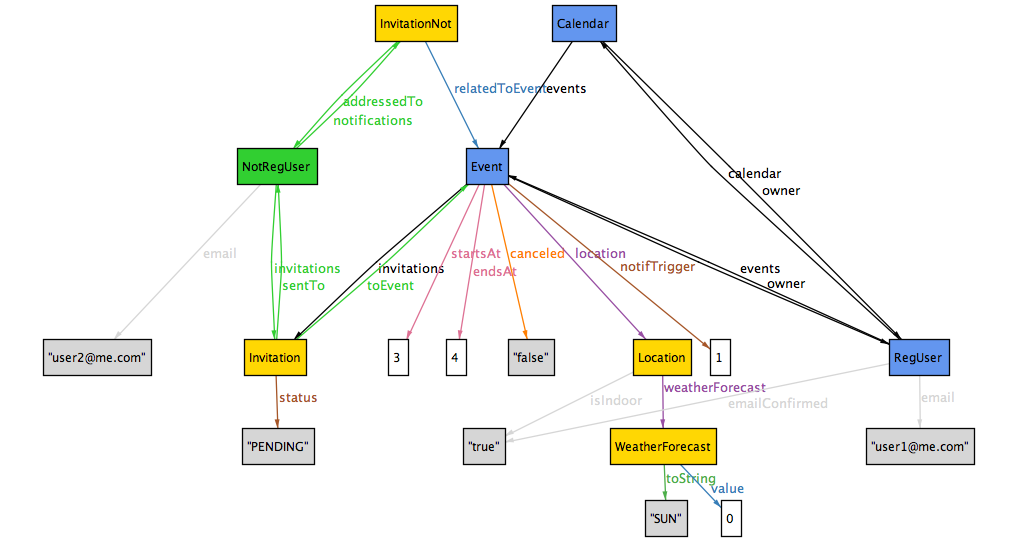
\includegraphics[scale=0.7]{World1}\footnote{Figure 1 : not registered user world}\\
\end{landscape}
\begin{landscape}
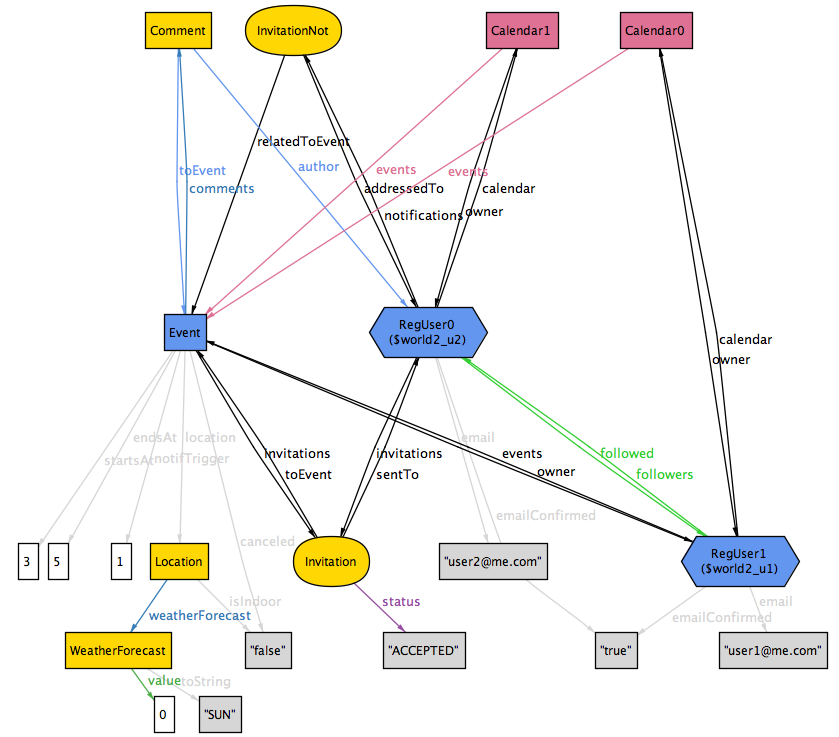
\includegraphics[scale=0.6]{World2}\footnote{Figure 2 : invitation world}\\
\end{landscape}
\begin{landscape}
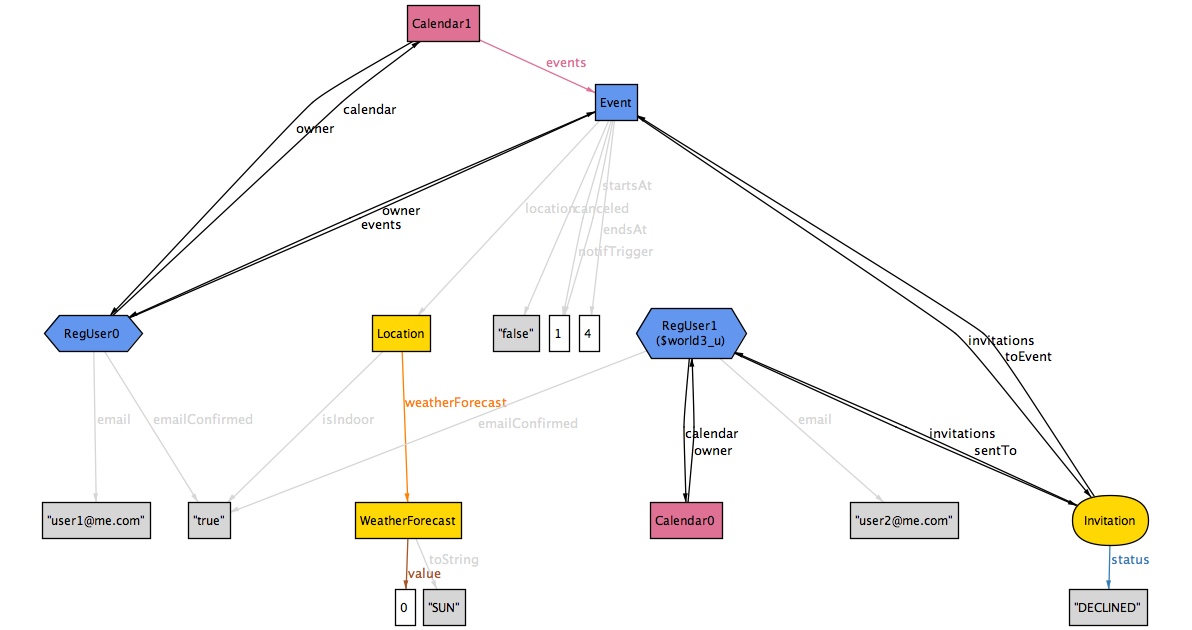
\includegraphics[scale=0.6]{World3}\footnote{Figure 1 : decline invitation world}\\
\end{landscape}
\begin{landscape}
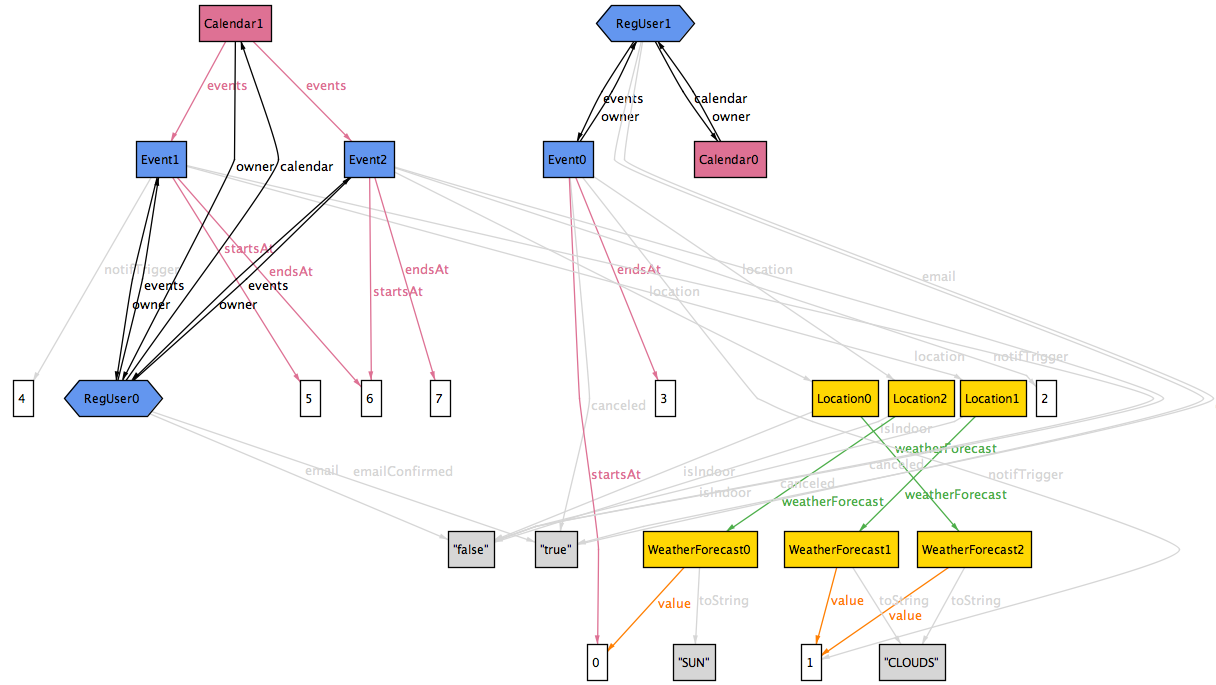
\includegraphics[scale=0.6]{World4}\footnote{Figure 2 :  concurrent event world}\\
\end{landscape}
\begin{landscape}
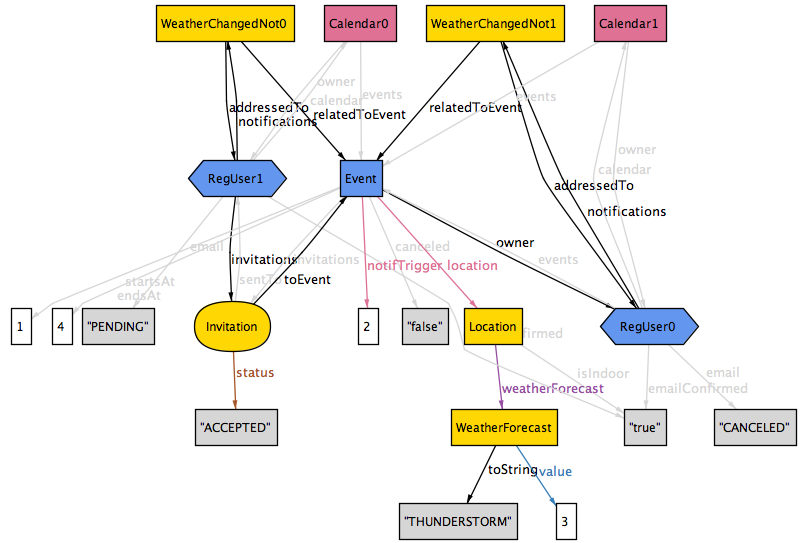
\includegraphics[scale=0.7]{World5}\footnote{Figure 1 : weather changed world}\\
\end{landscape}



\chapter{Used Tools}

Tools we used to create this RASD document are the following : 
\begin{itemize}
	\item LaTeX: to write and format this document
	\item Pages : to draw extra figures and graphs
	\item Signavio Platform : to design Use Cases
	\item starUML : to design Class Diagrams and State Charts Diagram
	\item Visual Paradigm : to design Sequence Diagrams
	\item Blasmiq Mockup : to design web pages' mockup
	
\end{itemize}

\chapter{References}

- SE2 teacher Mirandola's lecture slides \\ 
- The Meaning of Requirements: \\$http://www.uml.org.cn/requirementproject/pdf/jackson\_annals97.pdf$ \\
- Non-functional Requirements : \\$http://en.wikipedia.org/wiki/Non-functional\_requirement$
\end{document}
